\part{Overview / Basics}
\label{p:overview}

In the first part of these notes, we describe different 
types of stochastic gravitational-wave backgrounds and 
introduce the
method of cross-correlation for extracting the signal
from noise.

\section{Motivation}
\label{s:motivation}

A stochastic background of gravitational radiation 
is a superposition of gravitational-wave signals that
are either too weak or too numerous to individually detect.
The individual signals making up the background are thus
{\em unresolvable}, unlike the large signal-to-noise 
binary black-hole (BBH) and binary neutron-star (BNS)
merger signals recently detected by the advanced LIGO 
and Virgo detectors.
But despite the fact that the individual signals are 
unresolvable, the detection of a gravitational-wave 
background (GWB) will provide information about the 
{\em statistical} properties (or population properties)
of the source.

\subsection{Gravitational-wave analogue of the cosmic
microwave background}
\label{s:GW_CMB}

The ultimate goal of GWB searches is to produce 
the GW analogue of Figure~\ref{f:CMB},
%
\begin{figure}[htbp!]
\begin{center}
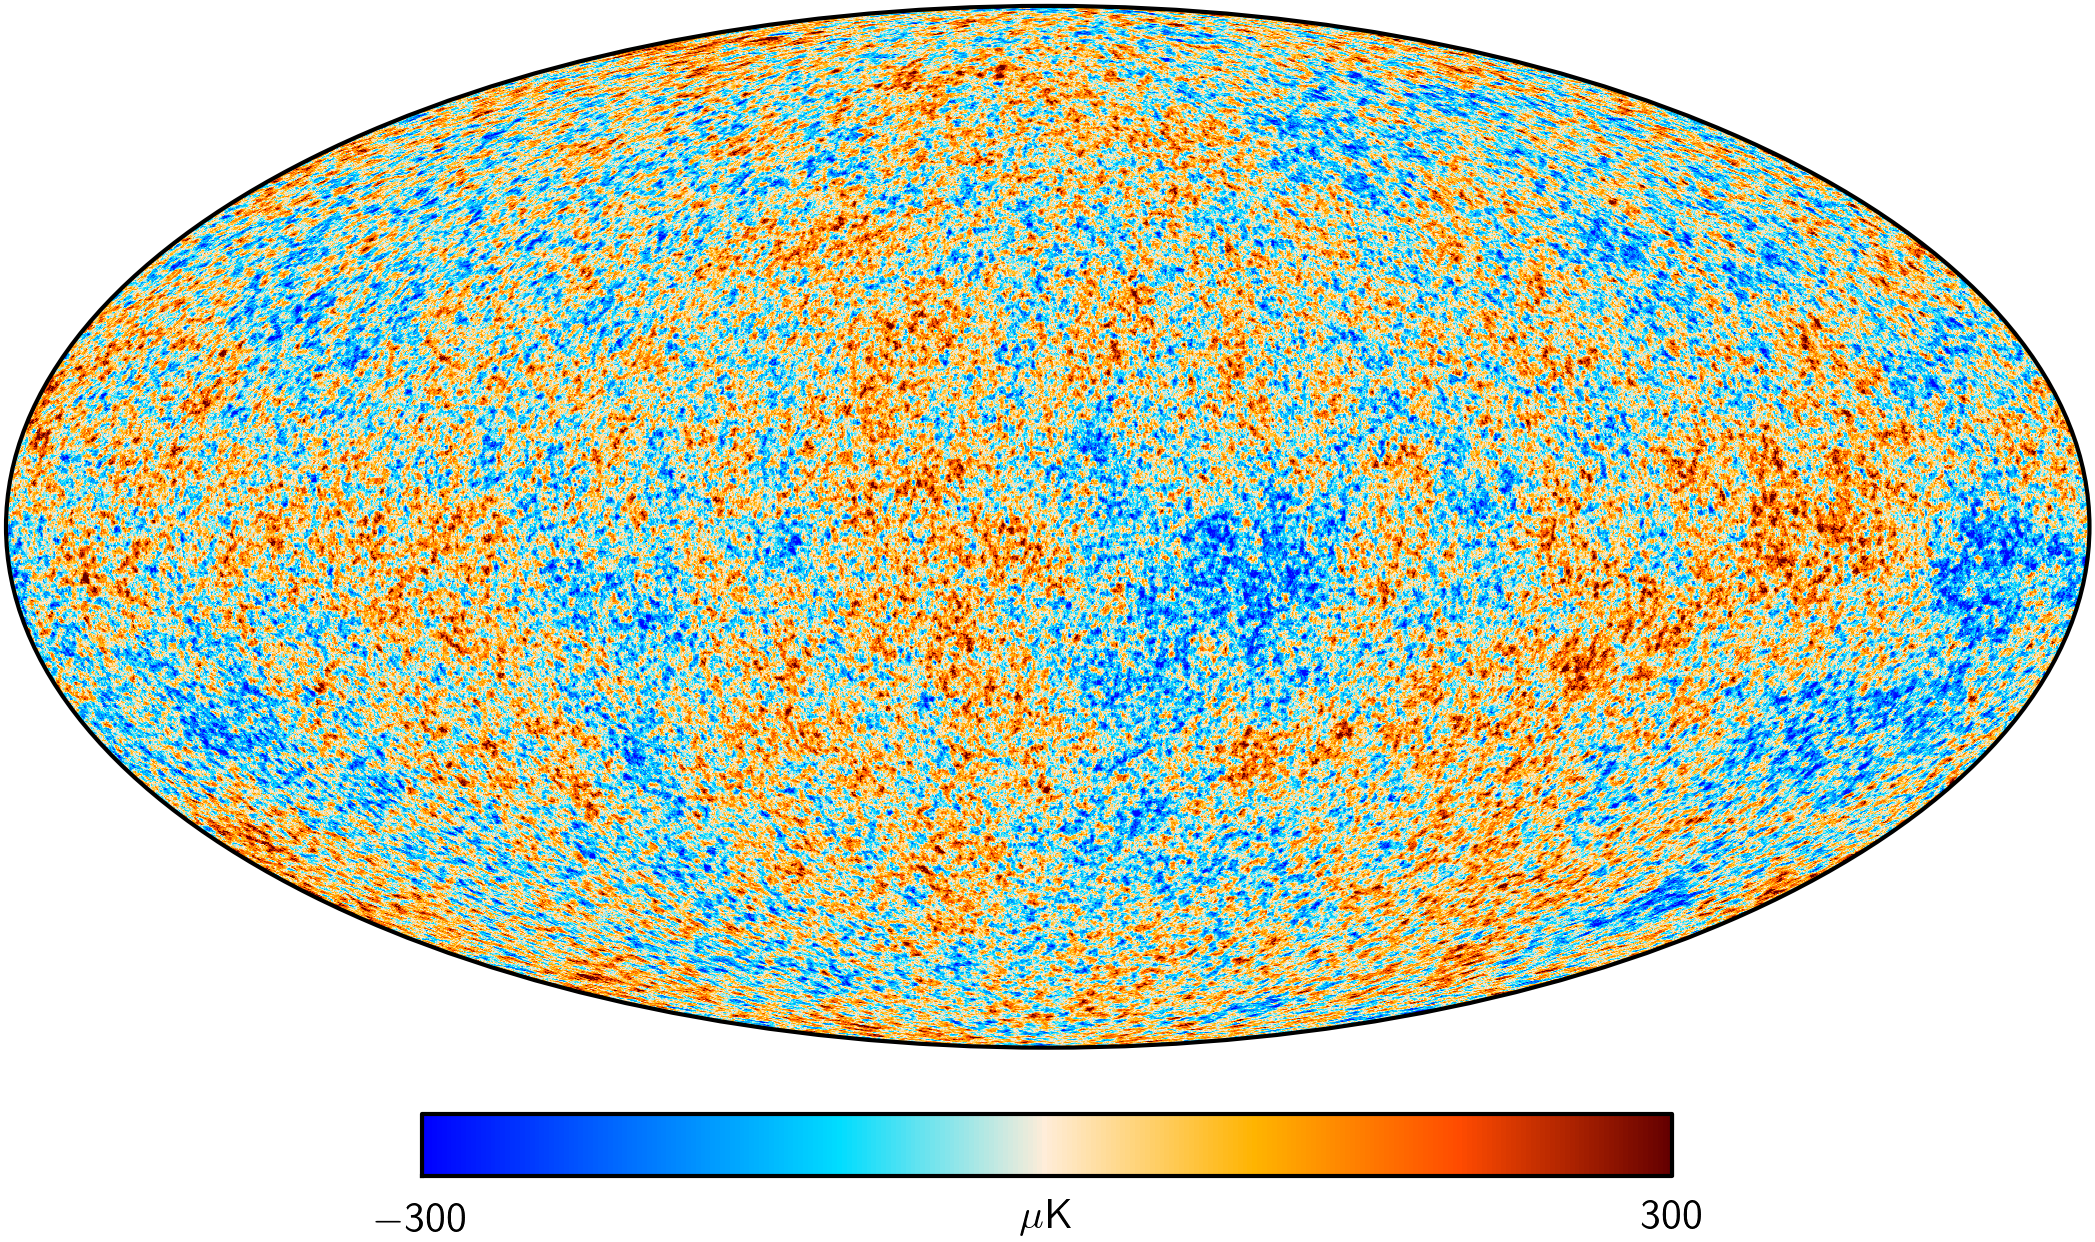
\includegraphics[width=0.6\textwidth]{Figures/CMB}
\caption{Skymap of $\Delta T/T_0$ for the cosmic microwave background
radiation produced by the Planck 2013 mission.}
\label{f:CMB}
\end{center}
\end{figure}
%
which is a sky map of the temperature fluctuations in 
the cosmic microwave background (CMB) 
blackbody radiation, $\Delta T/T_0$, relative 
to the $T_0 = 2.73~{\rm K}$ isotropic component.
(The dipole contribution due to our motion with respect 
to the cosmic rest frame has also been subtracted out.)
The CMB is a background of electromagnetic
radiation, produced roughly 380,000~yr after the Big Bang.
At that time, the universe had a temperature of 
$\sim 3000~{\rm K}$, approximately one thousand times 
larger than the temperature today, but cool enough for 
neutral hydrogen atoms to first form and photons to 
propagate freely.
The temperature fluctuations in the CMB radiation tell
us about the density perturbations at the time of 
last scattering of photons, 
thus giving us a picture of the ``seeds" of 
large-scale structure formation in the early universe.
Given the weakness of the gravitational interaction 
compared to the electromagnetic force, the GW analogue 
of Figure~\ref{f:CMB} would provide information about
a much earlier time in the evolution of the universe,
a mere fraction of a second after the Big Bang 
(this is explained in a bit more detail in 
Section~\ref{s:different_sources}).  
Detecting the cosmological GWB is thus a ``holy grail" 
for GW astronomy.

For perspective, Figure~\ref{f:CMB} was produced by 
the Planck mission in 2013,
almost 50 years after the CMB radiation was initially
detected by Penzias and Wilson in 1965.
It took many years and improved experiments
(COBE, Boomerang, WMAP, Planck to name a few) to get to 
the high-precision measurements that we have today.
So it is somewhat sobering to realize that now---at the 
end of 2018---we have yet to detect the isotropic component 
of the GWB.

\subsection{The background of BBH and BNS mergers in the 
LIGO band}
\label{s:BBH-BNS-LIGO}

Even though a detailed map of the primordial GWB is likely
to be out of reach for many years, there are other
sources of GWBs that are much more immediately accessible
to us.
For example, as mentioned above, the advanced LIGO
and Virgo detectors have detected other 
gravitational-wave signals from several individual BBH 
and BNS mergers.
These were very strong signals, having 
matched-filter signal-to-noise ratios (SNR) $\gtrsim 10$, 
and false alarm probabilities $<2\times 10^{-7}$,
corresponding to 5-sigma ``gold-plated" events.
Similar large-SNR detections are expected during the 
observing run O3, which started on 1 April 2019.
But we also expect that there are many more signals, 
corresponding to more distant mergers or smaller mass systems, 
which are 
individually undetectable (i.e., {\em subthreshold} events).
This weaker background of gravitational radiation is 
nonetheless detectable as a combined/aggregate signal
via the common influence of the component GWs on 
multiple detectors.

To get an idea of the statistical properties of this
background signal, we can estimate the total rate of 
stellar-mass BBH mergers throughout the universe by
using the local rate estimate from these first detections,
$9$-$240~{\rm Gpc}^{-3}\,{\rm yr}^{-1}$.
This leads to a prediction for the total rate of 
BBH mergers between $\sim\!1$~per minute to a few per hour.
(You are asked in Exercise~\ref{exer:1} to verify
these predictions.)%
\footnote{A more complete description of this and 
all other exercises are given in 
Section~\ref{s:exercises}.
The number next to ``Exercise" is a link that brings 
you to the detailed exercise in Section~\ref{s:exercises}.}
Since the duration of BBH merger signals in band 
is $\sim\!1~{\rm s}$, which is much smaller than the 
average duration between successive mergers, the 
combined signal will consist of discrete bursts of 
radiation separated by periods of silence 
(i.e., it will be {\em popcorn}-like).
We can perform similar calculations for BNS mergers.
The predicted total rate for such events is roughly 
one event every $15~{\rm s}$, while the duration of 
a BNS signal in band is roughly 100~{\rm s}. 
Thus, the BNS merger signals overlap in time leading to 
a continuous (or {\em confusion-limited}) background.
Figure~\ref{f:BBH-BNS-timeseries} is a plot of the
expected time-domain signal corresponding to the rate
estimates mentioned above.
%
\begin{figure}[htbp!]
\begin{center}
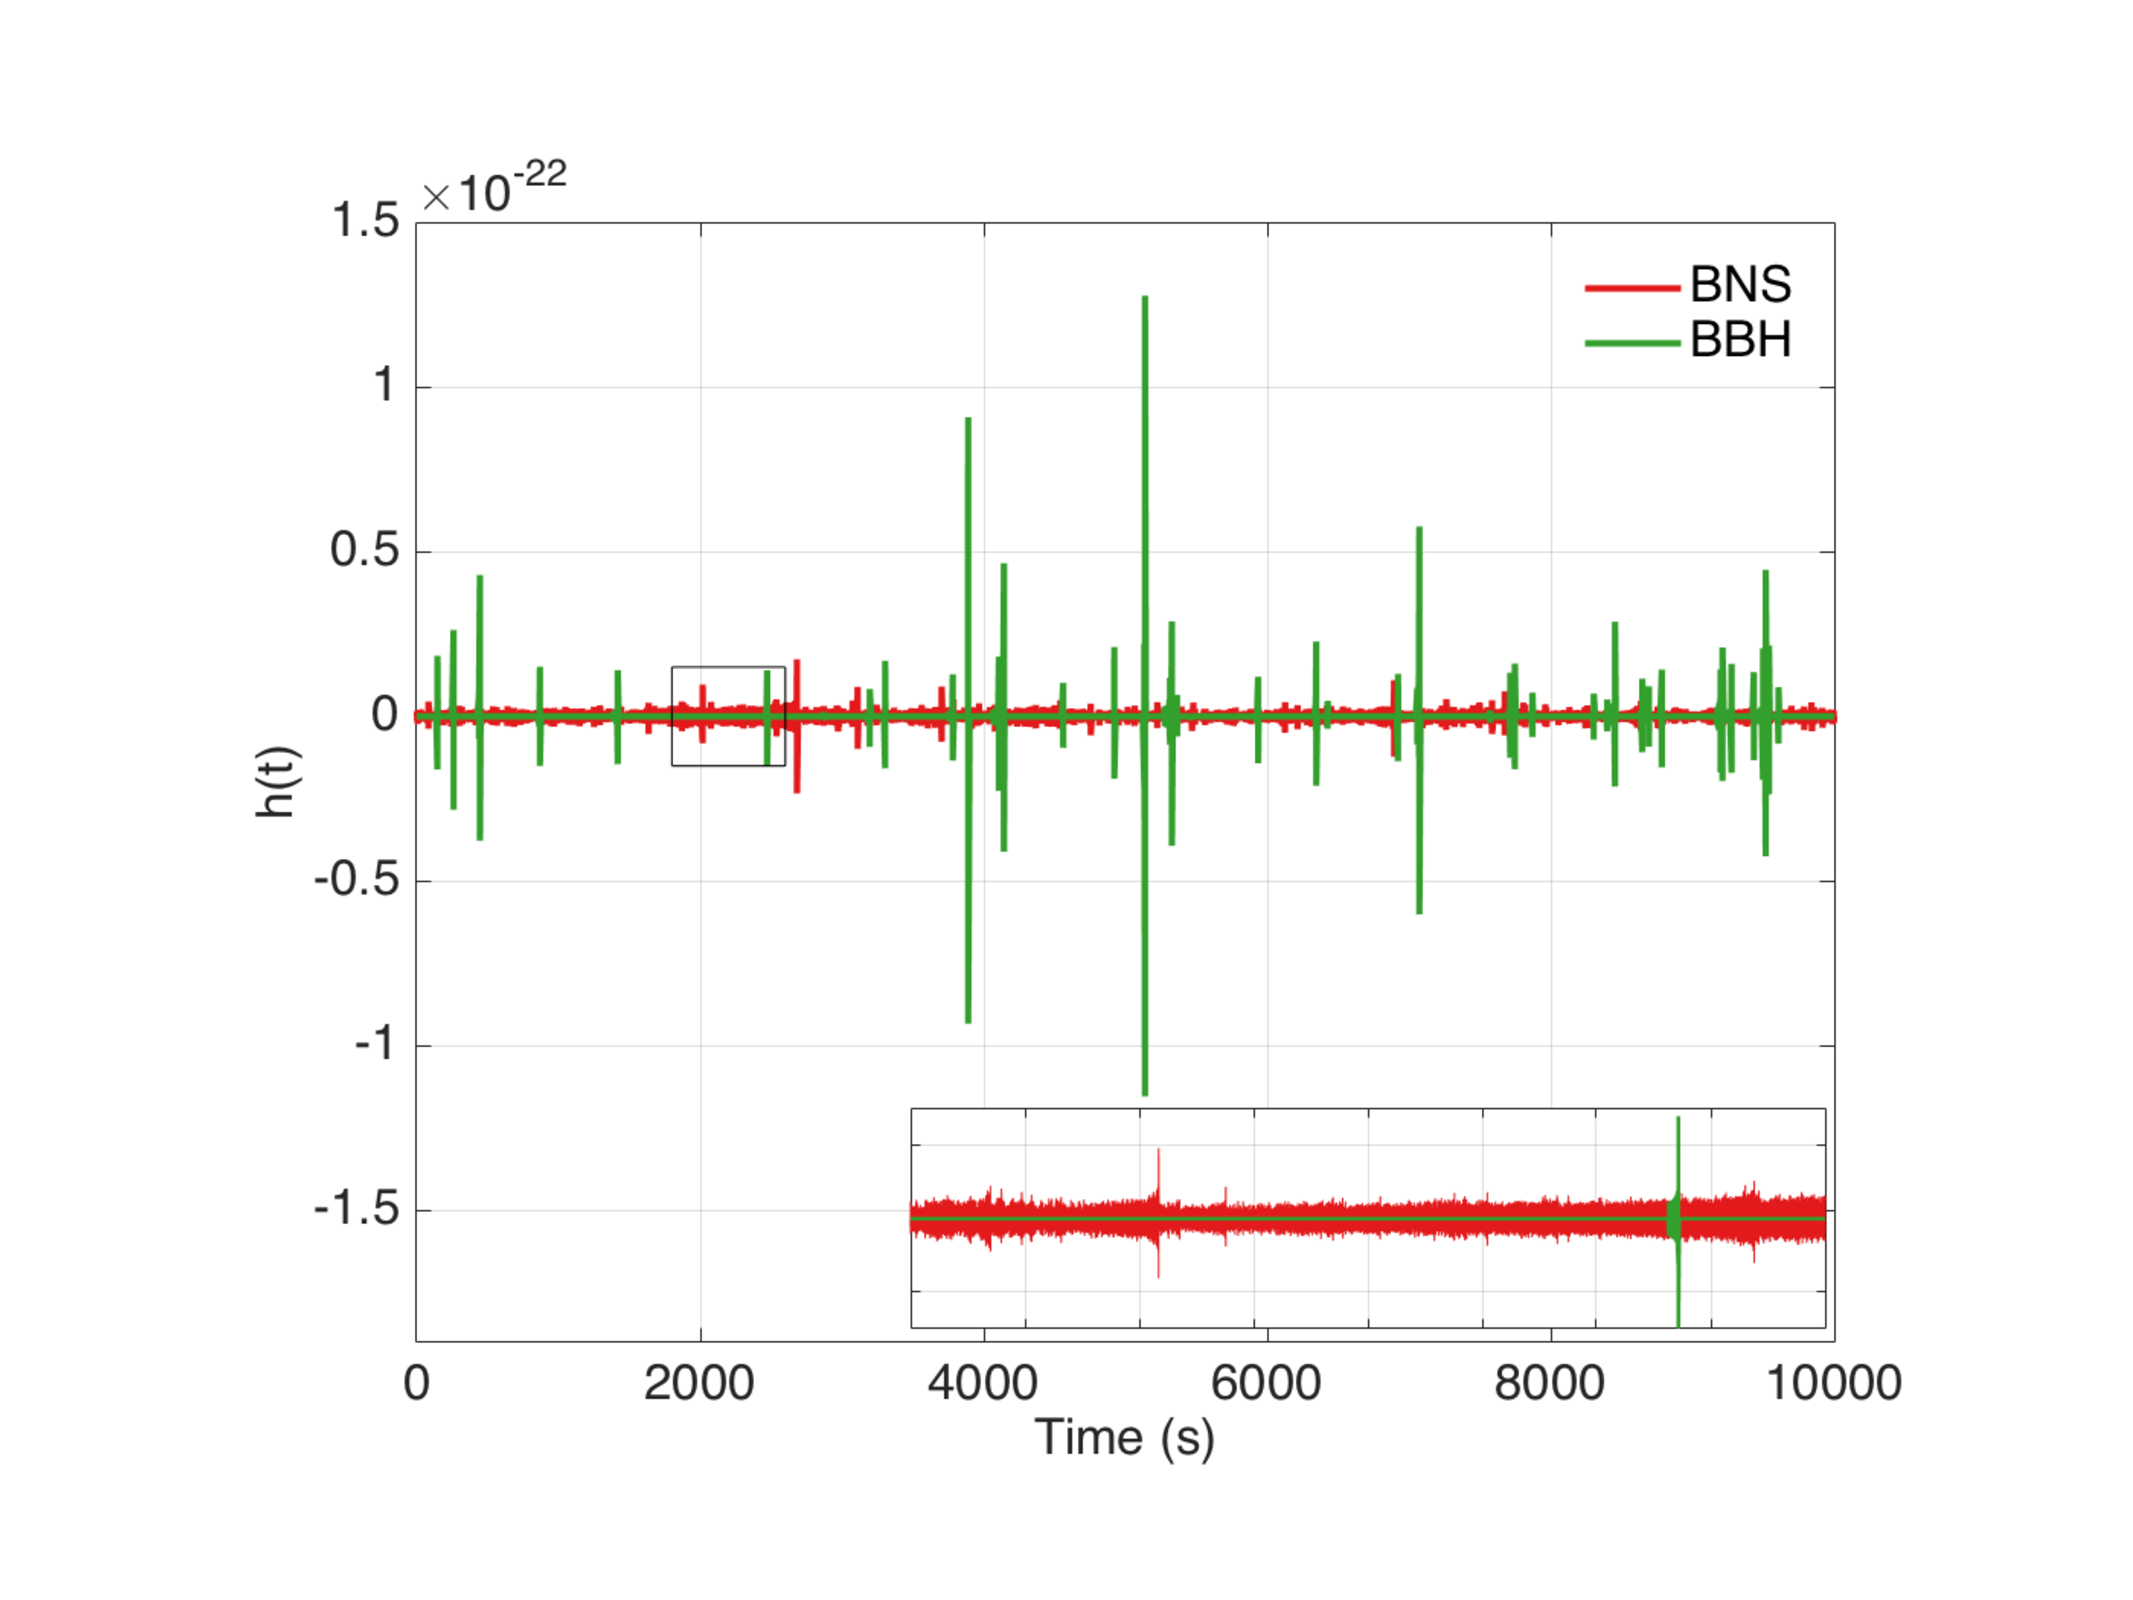
\includegraphics[width=0.7\textwidth]{Figures/BBH-BNS-timeseries}
\caption{Simulated time-domain signal for the predicted BBH and 
BNS background.  
Figure taken from \cite{stoch-implications}.}
\label{f:BBH-BNS-timeseries}
\end{center}
\end{figure}
%

The combined signal from BBH and BNS mergers is 
potentially detectable with advanced LIGO and Virgo, 
shortly after reaching design sensitivity.
Although the signal-to-noise ratios for the 
individual events are small, the combined 
signal-to-noise ratio of the correlated data 
summed over all events grows like the square-root 
of the observation time, reaching a detectable
level of $3$-sigma after roughly 40~months of
observation (Figure~\ref{f:BBH-BNS-SNR}).
%
\begin{figure}[htbp!]
\begin{center}
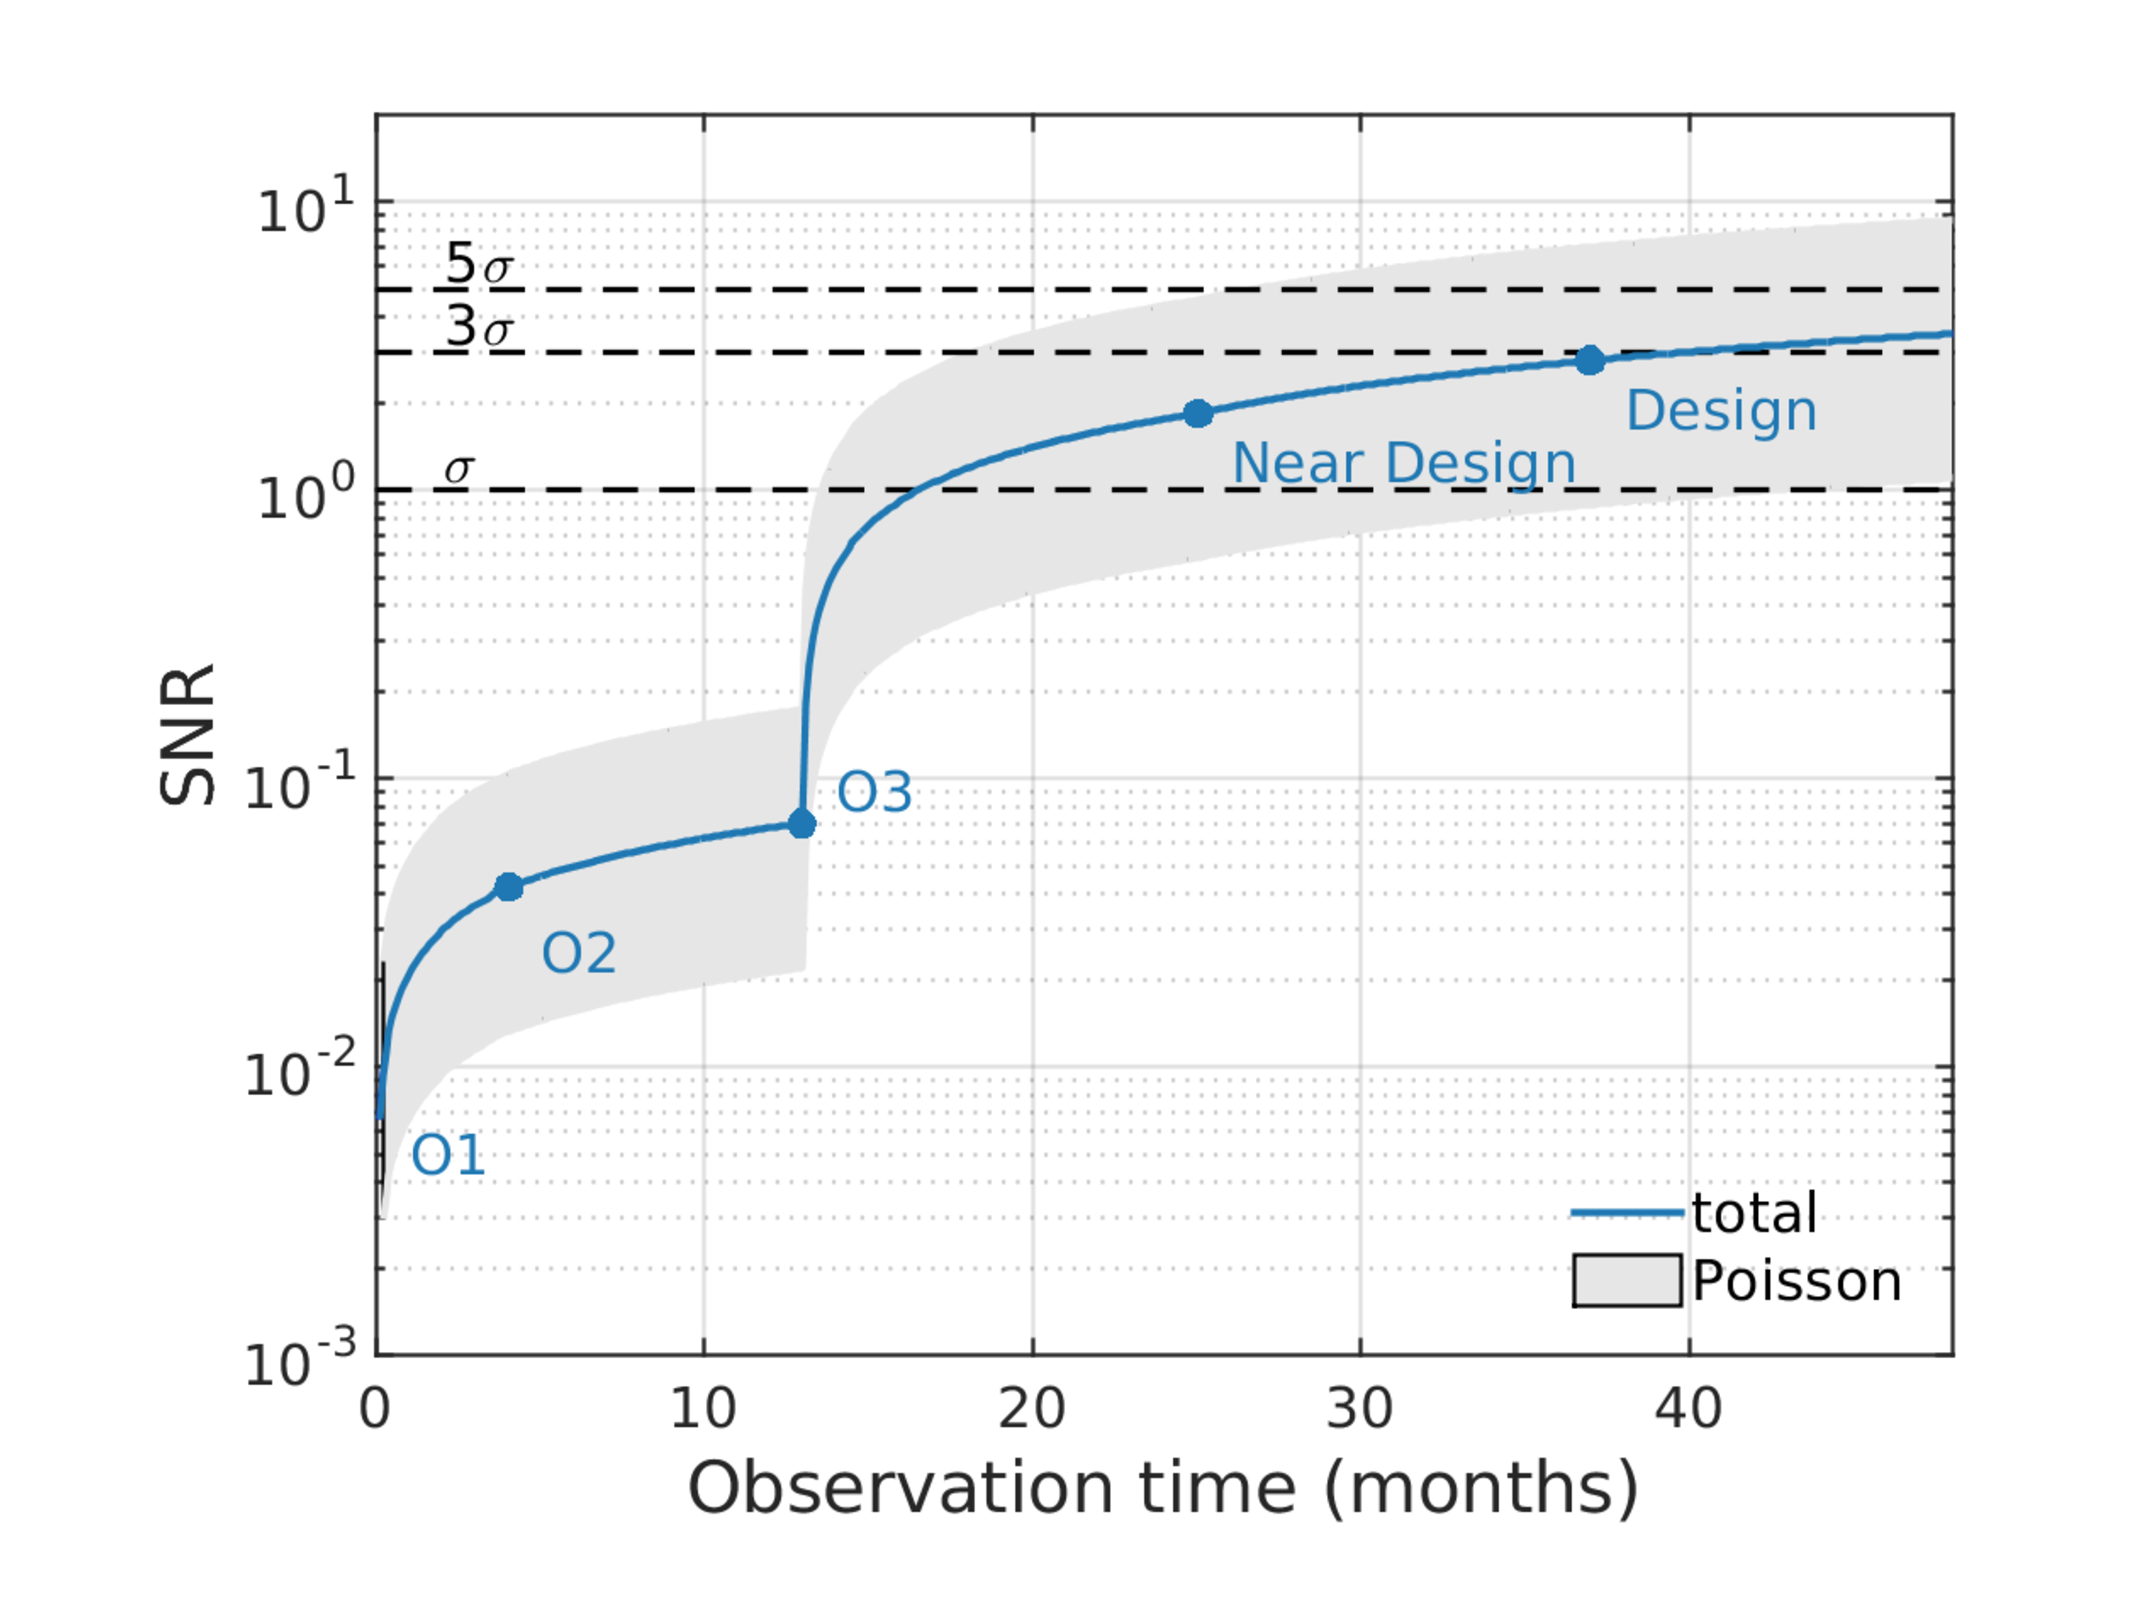
\includegraphics[width=0.7\textwidth]{Figures/BBH-BNS-SNR}
\caption{Expected signal-to-noise ratio of the correlated 
data for the advanced LIGO and Virgo detectors as a function 
of observation time.
The points labeled O1, O2, etc., indicate the start of
advanced LIGO's first observation run, second observation
run, etc. 
Figure taken from \cite{stoch-implications}.}
\label{f:BBH-BNS-SNR}
\end{center}
\end{figure}
%
This estimate of time to detection is based on 
the standard cross-correlation search (Section~\ref{s:correlations}), 
which assumes a Gaussian-stationary background.
But there is a new method, recently proposed by 
Smith and Thrane~\cite{Smith-Thrane:2019}, 
which can potentially reduce the time to detection by several 
orders of magnitude (factor of $\sim\!1000$), 
meaning that the background would be detectable after only
a few days of operation. 
We will describe this method in more detail in 
Section~\ref{s:nonstationary}.

%%%%%%%%%%%%%%%%%%%%%%%%%%%%%%%%%%%%%%%%%%%%%%%%%%%%%%%
\section{Different types of stochastic backgrounds}
\label{s:different_types}

\subsection{Different sources}
\label{s:different_sources}

The combined signal from stellar-mass BBH and BNS 
mergers throughout the universe is just one way 
of producing a GWB.
Due to the relatively small masses of stellar-mass 
BHs and NSs, the signal is at the high-frequency 
end of the spectrum ($\sim\!10~{\rm Hz}$ to a few kHz), 
which is the sensitive band for the current generation 
of km-scale ground-based laser interferometers like 
LIGO and Virgo.
Heavier-mass systems, which produce lower-frequency 
gravitational waves, are also expected to give rise 
to GWBs that are potentially detectable with other 
existing or proposed detectors.
Figure~\ref{f:GWspectrum} is a plot of the GW 
spectrum, with frequencies ranging
from a few kHz (for ground-based detectors)
to $10^{-17}~{\rm Hz}$ (corresponding to a period
equal to the age of the universe), together with 
potential sources of GWBs and relevant detectors.  
%
\begin{figure}[htbp!]
\begin{center}
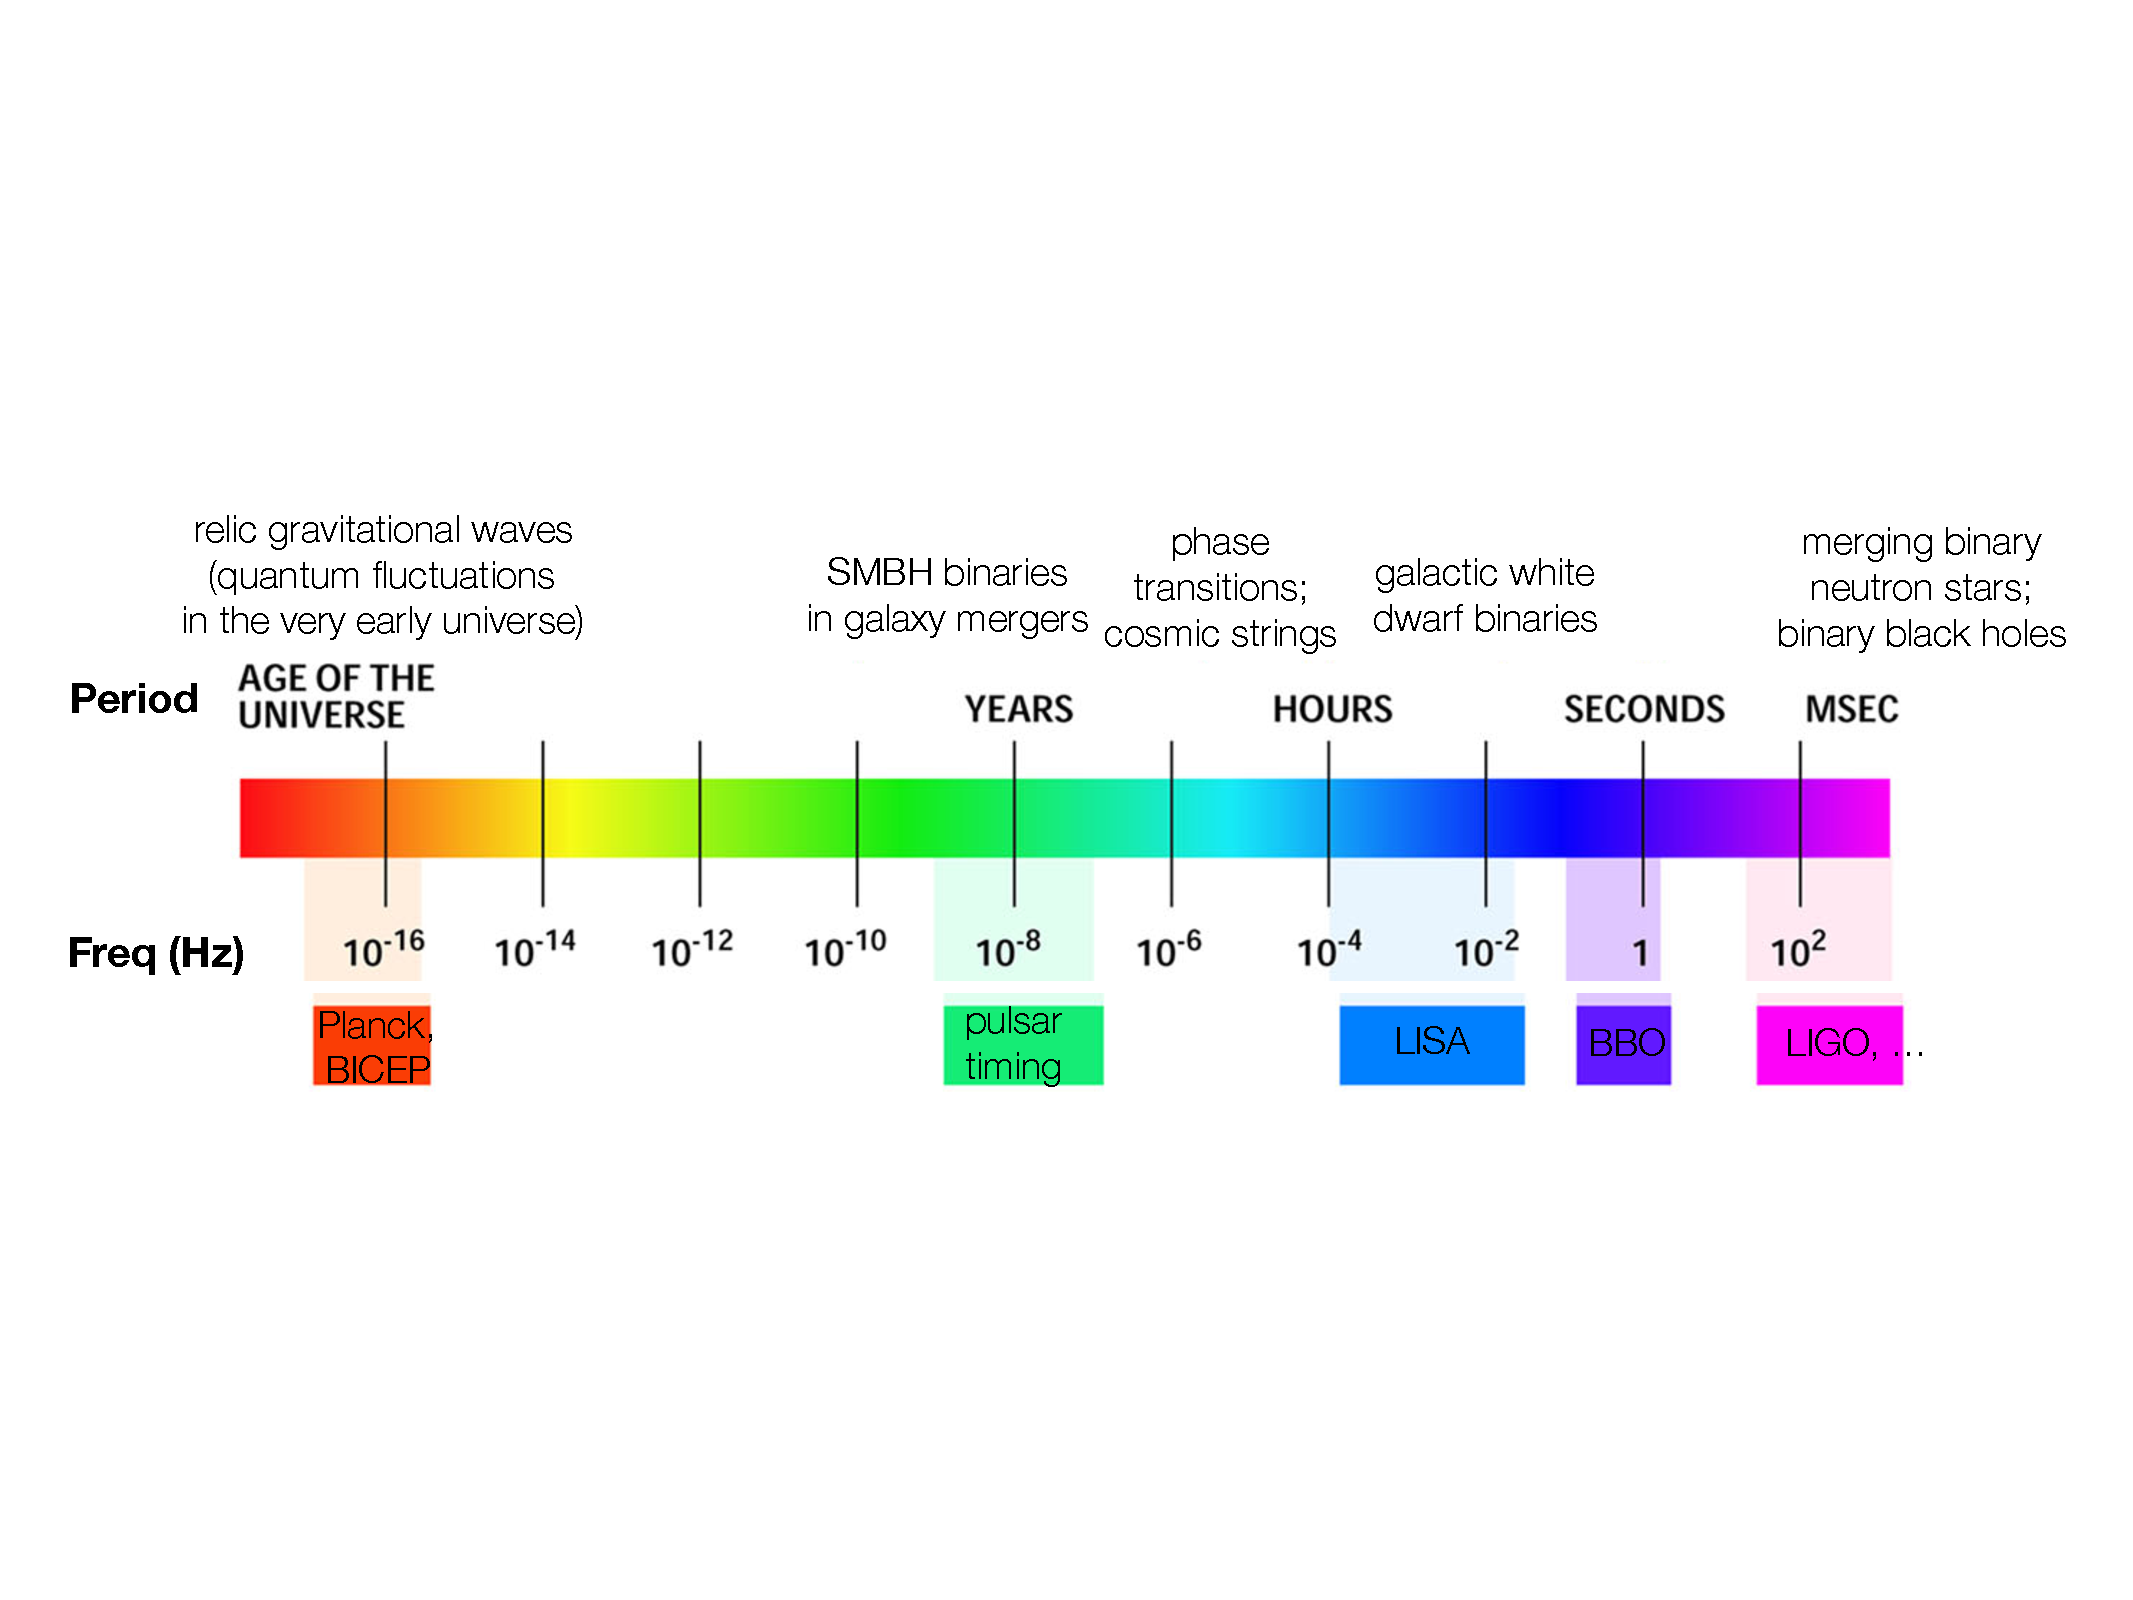
\includegraphics[width=\textwidth]{Figures/GWspectrum}
\caption{Detectors and potential sources of GWBs
across the GW spectrum.
Note that the GWB signal from cosmic strings and phase 
transitions stretch across a broad range of frequencies, 
and peak at basically any frequency depending on 
the parameters that define the string network and the 
energy scale where the phase transition occurs.
Also, the primordial background of relic GWs predicted 
by standard inflation is flat across the whole frequency 
band shown here.}
\label{f:GWspectrum}
\end{center}
\end{figure}
%

Of particular note is the combined GW 
signal produced by compact white-dwarf binaries in 
the Milky Way, producing a ``confusion-limited" GWB
in the frequency band $\sim 10^{-4}~{\rm Hz}$ to 
$10^{-1}~{\rm Hz}$.
This is a guaranteed signal for the proposed 
space-based interferometer LISA (expected launch date 2034), 
which consists of three spacecraft in an 
equilaterial-triangle configuration 
in orbit around the Sun.
Each spacecraft houses two lasers, two telescopes, and 
two test masses; 
the arms will be several million km long.
The confusion-limited 
white-dwarf binary signal is expected to be 
so strong that it will
dominate the instrumental noise at low frequencies, 
forming a GW ``foreground" that will
have to be contended with when searching for other 
gravitational sources in the LISA band.

At lower frequencies between 
$\sim\!10^{-9}~{\rm Hz}$ and $10^{-7}~{\rm Hz}$
(corresponding to periods of order decades to years), 
pulsar timing arrays can be used to 
search for the GWB produced by the inspiral and merger 
of supermassive black-holes (SMBHs) in the centers of
distant galaxies.
A pulsar timing array basically functions as a 
galactic-scale gravitational-wave detector, with the
radio pulses emitted by each pulsar behaving like 
`ticks' of an extremely stable clock.
By carefully monitoring the arrival times of these
radio pulses, one can search for a GWB by looking for 
correlated modulations in the arrival times 
induced by a passing gravitational wave.

In addition to these {\em astrophysical} GWBs 
associated with stellar-mass or supermassive BHs 
and NSs, one also expects backgrounds of 
{\em cosmological} origin, produced in the 
very early universe, much before the formation of 
stars and galaxies.  
Two examples, indicated in Figure~\ref{f:GWspectrum}, 
are cosmic strings (line-like topological defects 
associated with 
phase transistions in the early universe) and
relic gravitational waves (quantum 
fluctuations in the geometry of space-time, 
driven to macroscopic scales by a period of rapid 
expansion---e.g., inflation---a mere 
$\sim\!10^{-32}~{\rm s}$ after the Big Bang).
This relic background is potentially detectable 
by its effect on the polarization of the CMB radiation.
This signal has been searched for by CMB experiments
such as Planck and BICEP, and is a core target of many
proposed future experiments, such as PIXIE and LiteBIRD.

\subsection{Different signal properties}
\label{s:different_signal_properties}

Not surprisingly, different sources of a GWB give
rise, in general, to different properties of the 
observed signal.
These differences are what will allow us to infer 
the source of the background from the measured signal.

(i) Stochastic backgrounds can differ from one another 
in terms of the angular distribution of 
gravitational-wave power on the sky.
Cosmologically-generated backgrounds, like those from 
cosmic strings or relic GWs,
are expected to be {\em statistically isotropic},
qualitatively similar to the CMB (Figure~\ref{f:CMB}).
The GW power in these backgrounds is {\em anisotropic}, 
following the spatial distribution of the particular
sources that produced it, but has no preferred 
direction when averaged over different realizations 
of the sources.
Different statistically isotropic backgrounds will
be characterized by different angular power spectra,
$C_l$ as a function of multipole moment $l$, where
%
\be
C(\theta) = \sum_{l=0}^\infty \frac{2l+1}{4\pi} 
C_l P_l(\cos\theta)\,,
\label{e:legendre_series}
\ee
%
is the angular correlation between the GW power 
coming from two directions $\hat n$ and $\hat n'$
separated by angle $\theta$.
If all of the $C_l$'s except the monopole, $C_0$, 
are equal to zero, then the GWB is said to be 
``exactly" isotropic.
Exact isotropy is the simplest mathematical model 
for stochastic backgrounds, and will be discussed
further in Section~\ref{s:ensemble_averages}.

Statistically isotropic backgrounds are to be contrasted
with {\em statistically anisotropic} backgrounds, 
whose distribution of power on the sky has preferred 
directions, even when averaged over different 
realizations of the sources that produce it.
For example, the ``confusion-limited" foreground that 
LISA will see from the population of close white-dwarf 
binaries in the Milky Way will have its GW
power concentrated in the direction of the Milky Way.
Figure~\ref{f:statiso-vs-aniso} shows simulated skymaps 
for a statistically isotropic background (left panel) and 
a statistically anisotropic background (right panel). 
The anisotropic background in that figure follows the
galactic plane in equatorial coordinates. 
%
\begin{figure}[htbp!]
\begin{center}
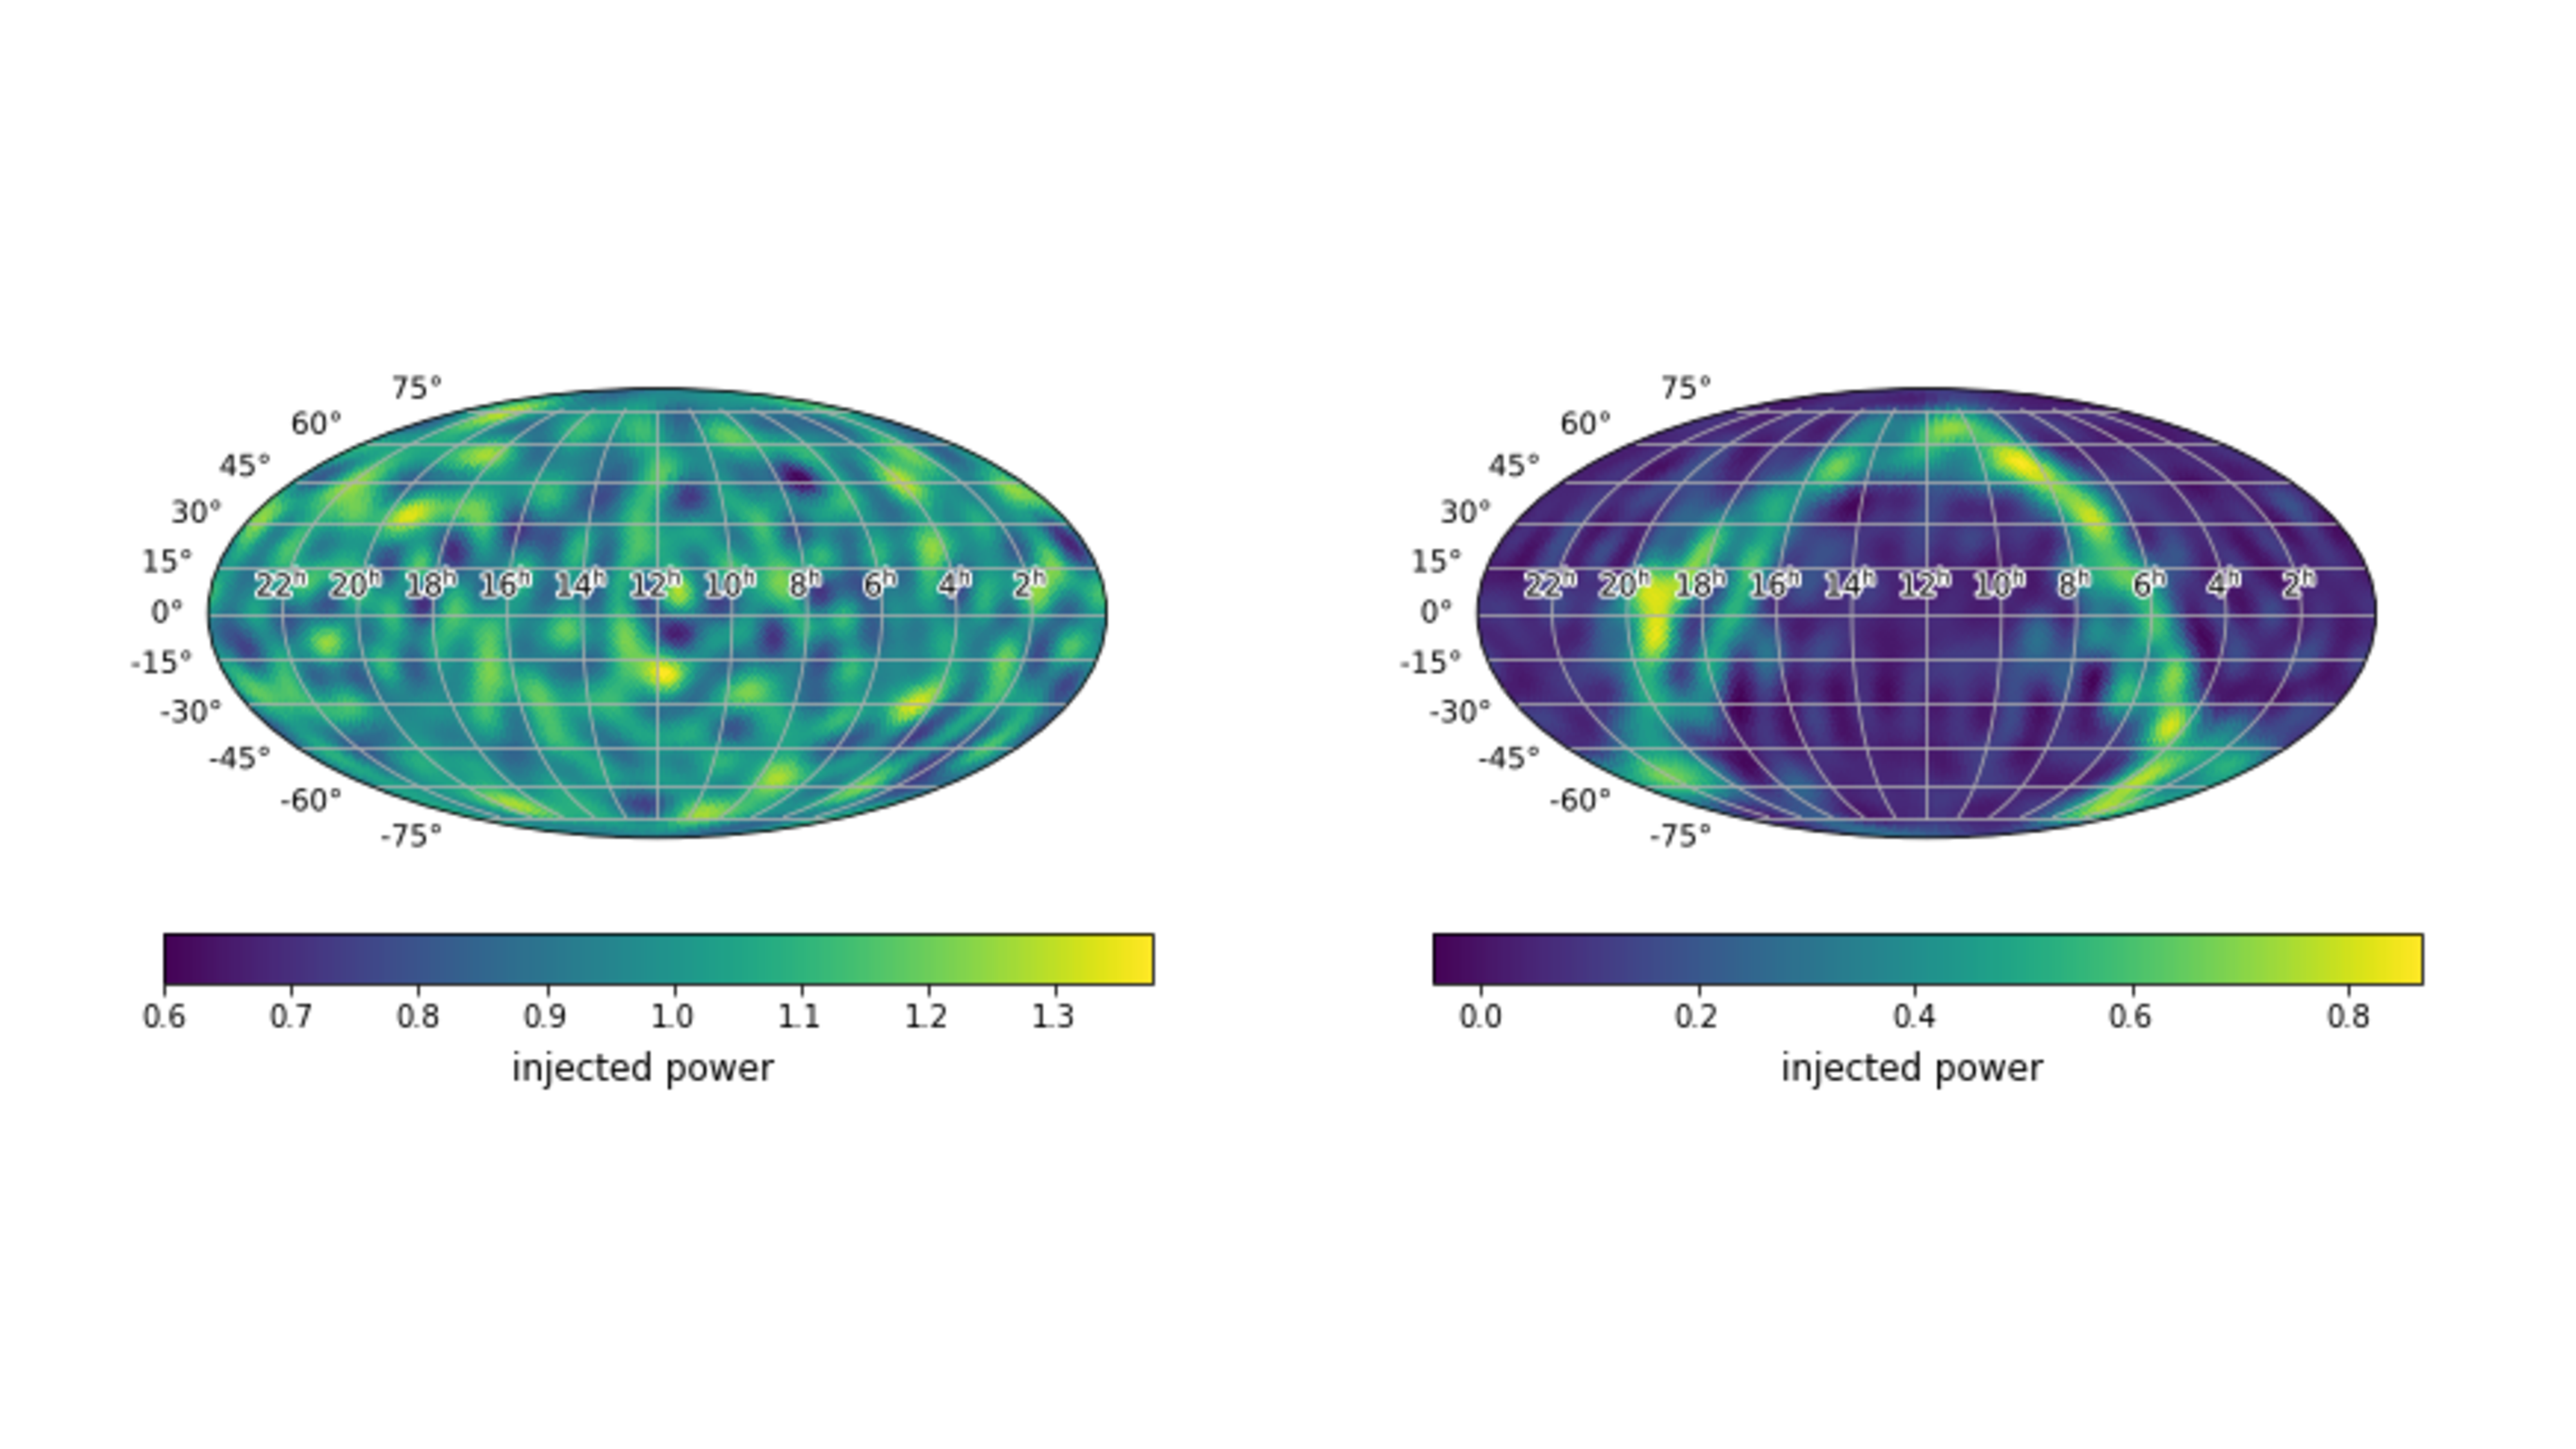
\includegraphics[width=\textwidth]{Figures/statiso-vs-aniso}
\caption{Simulated sky maps of gravitational-wave power
for a statistically isotropic background (left panel) and an 
anisotropic background (right panel).}
\label{f:statiso-vs-aniso}
\end{center}
\end{figure}
%

(ii) Stochastic backgrounds can also differ from one 
another in temporal distribution and amplitude.
We have already seen examples of this in 
Figure~\ref{f:BBH-BNS-timeseries}, for the expected
backgrounds from stellar-mass BBH mergers and 
BNS mergers throughout the universe (a LIGO source).
As mentioned earlier, the rate estimates and 
durations of these individual merger signals are such 
that the BBH background is expected to be popcorn-like 
(consisting of non-overlapping mergers), 
while that for the BNS background is expected to be
stationary and confusion-limited 
(consisting of several overlapping BNS mergers at any
instant of time).
Another example of non-trivial temporal dependence
is the confusion-limited signal from close 
white-dwarf binaries in the Milky Way (a LISA source).
This is an amplitude-modulated signal with 
a 6-month period (Figure~\ref{f:cyclostationary_data}), 
%
\begin{figure}[htbp!]
\begin{center}
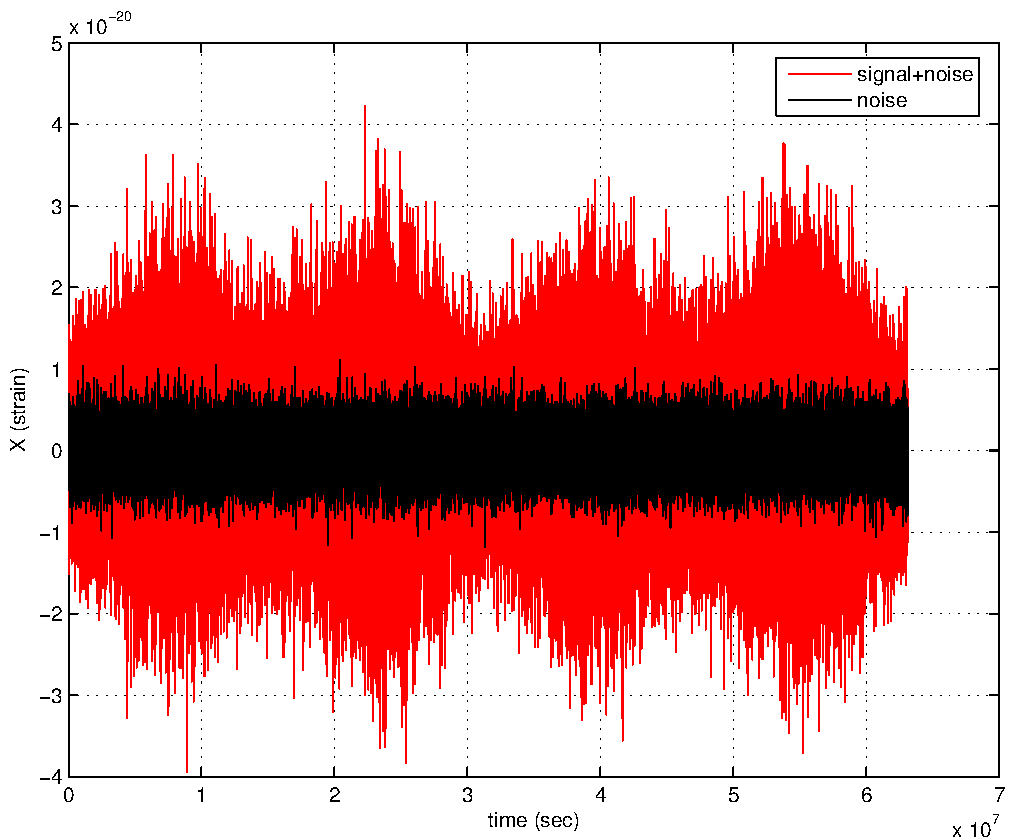
\includegraphics[width=0.6\textwidth]{Figures/cyclostationary_data}
\caption{Simulated time-domain output of a particular 
combination of the LISA data over a 2-year period.
The modulation of the signal with a 6-month period
is apparent in the data.
Figure taken from \cite{Romano-Cornish:2017}.}
\label{f:cyclostationary_data}
\end{center}
\end{figure}
%
due to LISA's ``cartwheeling" orbital motion around 
the Sun.
(The antenna pattern of LISA will point in the direction
of the Galactic center twice every year.) 
From the figure, we also see that the expected 
white-dwarf binary signal will be larger than that 
of the instrumental noise for LISA, thus constituting 
an astrophysical {\em foreground}.
This is atypical, however, as most expected GWBs will sit 
below the instrumental noise (e.g., for advanced LIGO / Virgo,
pulsar timing, CMB polarization experiments), requiring 
observation over long periods of time to confidently detect.

(iii) Stochastic backgrounds can also differ in their power 
spectra%
\footnote{Recall that if $x(t)$ is stationary time-domain data, 
then the power spectrum $P_x(f)$ is defined as the Fourier 
transform of the correlation function 
$C(t-t') \equiv \langle x(t)x(t')\rangle$, or,
equivalently, $\langle \tilde x(f)\tilde x^*(f')\rangle =
\frac{1}{2}P_x(f)\,\delta(f-f')$, where $\tilde x(f)$ is the Fourier
transform of $x(t)$.
See also Eq.~(\ref{e:quad_iso}).}
as shown in Figure~\ref{f:different_power_spectra}.
%
\begin{figure}[htbp!]
\begin{center}
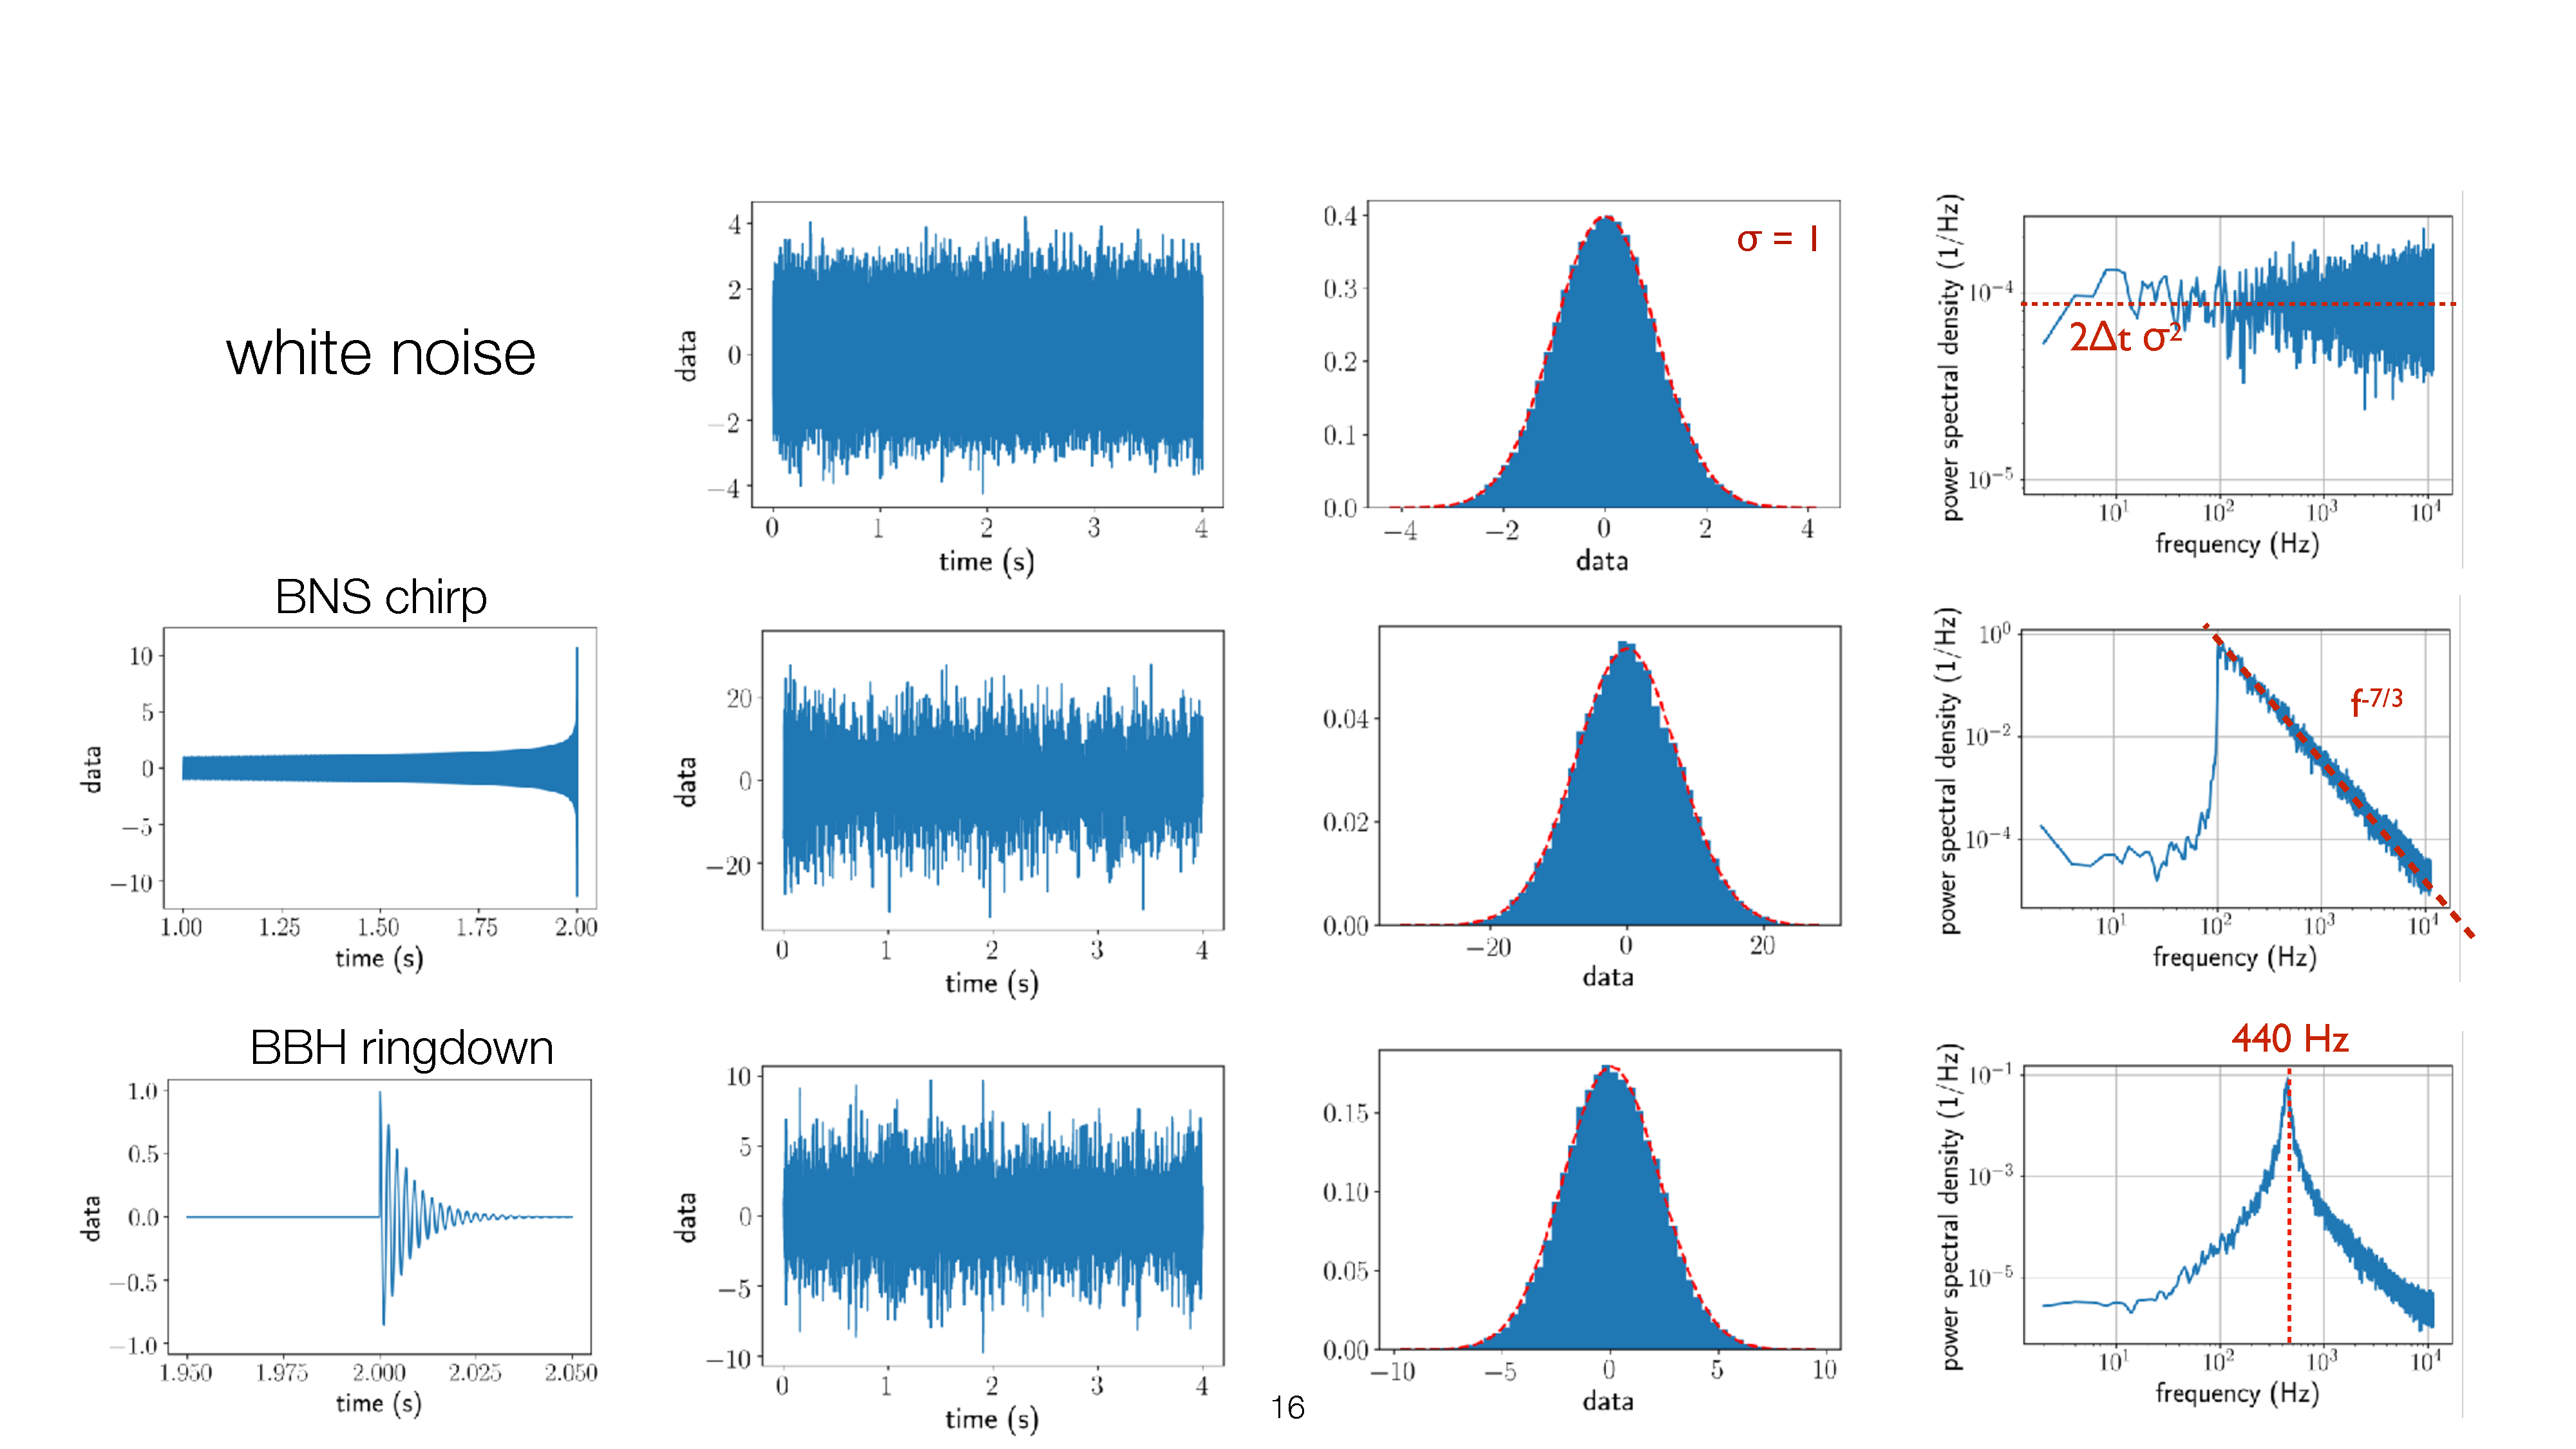
\includegraphics[width=\textwidth]{Figures/different_power_spectra}
\caption{Simulated time-domain data (including the signals for an
individual BNS merger and BBH ringdown), histograms, and power spectra
for three different types of Gaussian-stationary GWBs.}
\label{f:different_power_spectra}
\end{center}
\end{figure}
%
Here we plot simulated time-domain data (including the signals for an
individaul BNS merger and BBH ringdown%
\footnote{Our toy-model simulation for BBH ringdown is simply a 
damped sinusoid with frequency 440~Hz.
It has the correct qualitative behavior for a BBH ringdown, but 
is not meant to be astrophysically realistic.}), 
histograms, and power spectra
for three different types of GWBs.
For these toy-model simulations, we overlapped a sufficient number of 
individual BNS merger and BBH ringdown signals to produce 
Gaussian-stationary confusion-limited GWBs
(second and third columns).
The difference between these backgrounds shows up in their power 
spectra (third column).
The power spectra for the BNS merger and BBH ringdown backgrounds 
have the same shape as those for an individual BNS merger or 
BBH ringdown, scaled by the total number of sources contributing 
to the background.

%%%%%%%%%%%%%%%%%%%%%%%%%%%%%%%%%%%%%%%%%%%%%%%%%%%%%%%
\section{Mathematical characterization of a stochastic background}
\label{s:mathematical_characterization}

Since the individual signals comprising a GWB 
background are either too weak or too numerous to 
individually detect, the combined signal for the 
background is for all practical purposes 
{\em random}, similar to noise in an single detector.
Hence, we need to describe the GWB {\em statistically}, 
in terms of moments 
(i.e., ensemble averages) of the metric perturbations 
describing the GWB.

\subsection{Plane-wave expansion}
\label{s:plane_wave}

Recall that gravitational waves are time-varying 
perturbations to the geometry of space-time, 
which propagate away from the source at the speed 
of light.
In transverse-traceless coordinates
$(t,\vec x)\equiv (t,x^a)$, where $a=1,2,3$,
the metric perturbations corresponding to a 
plane wave (propagating in direction $\hat k\equiv-\hat n$) 
have two degrees of freedom, corresponding to the 
amplitudes of the 
plus ($+$) and cross ($\times$) polarizations of
the gravitational wave (Figure~\ref{f:polarizations}).
%
\begin{figure}[htbp!]
\begin{center}
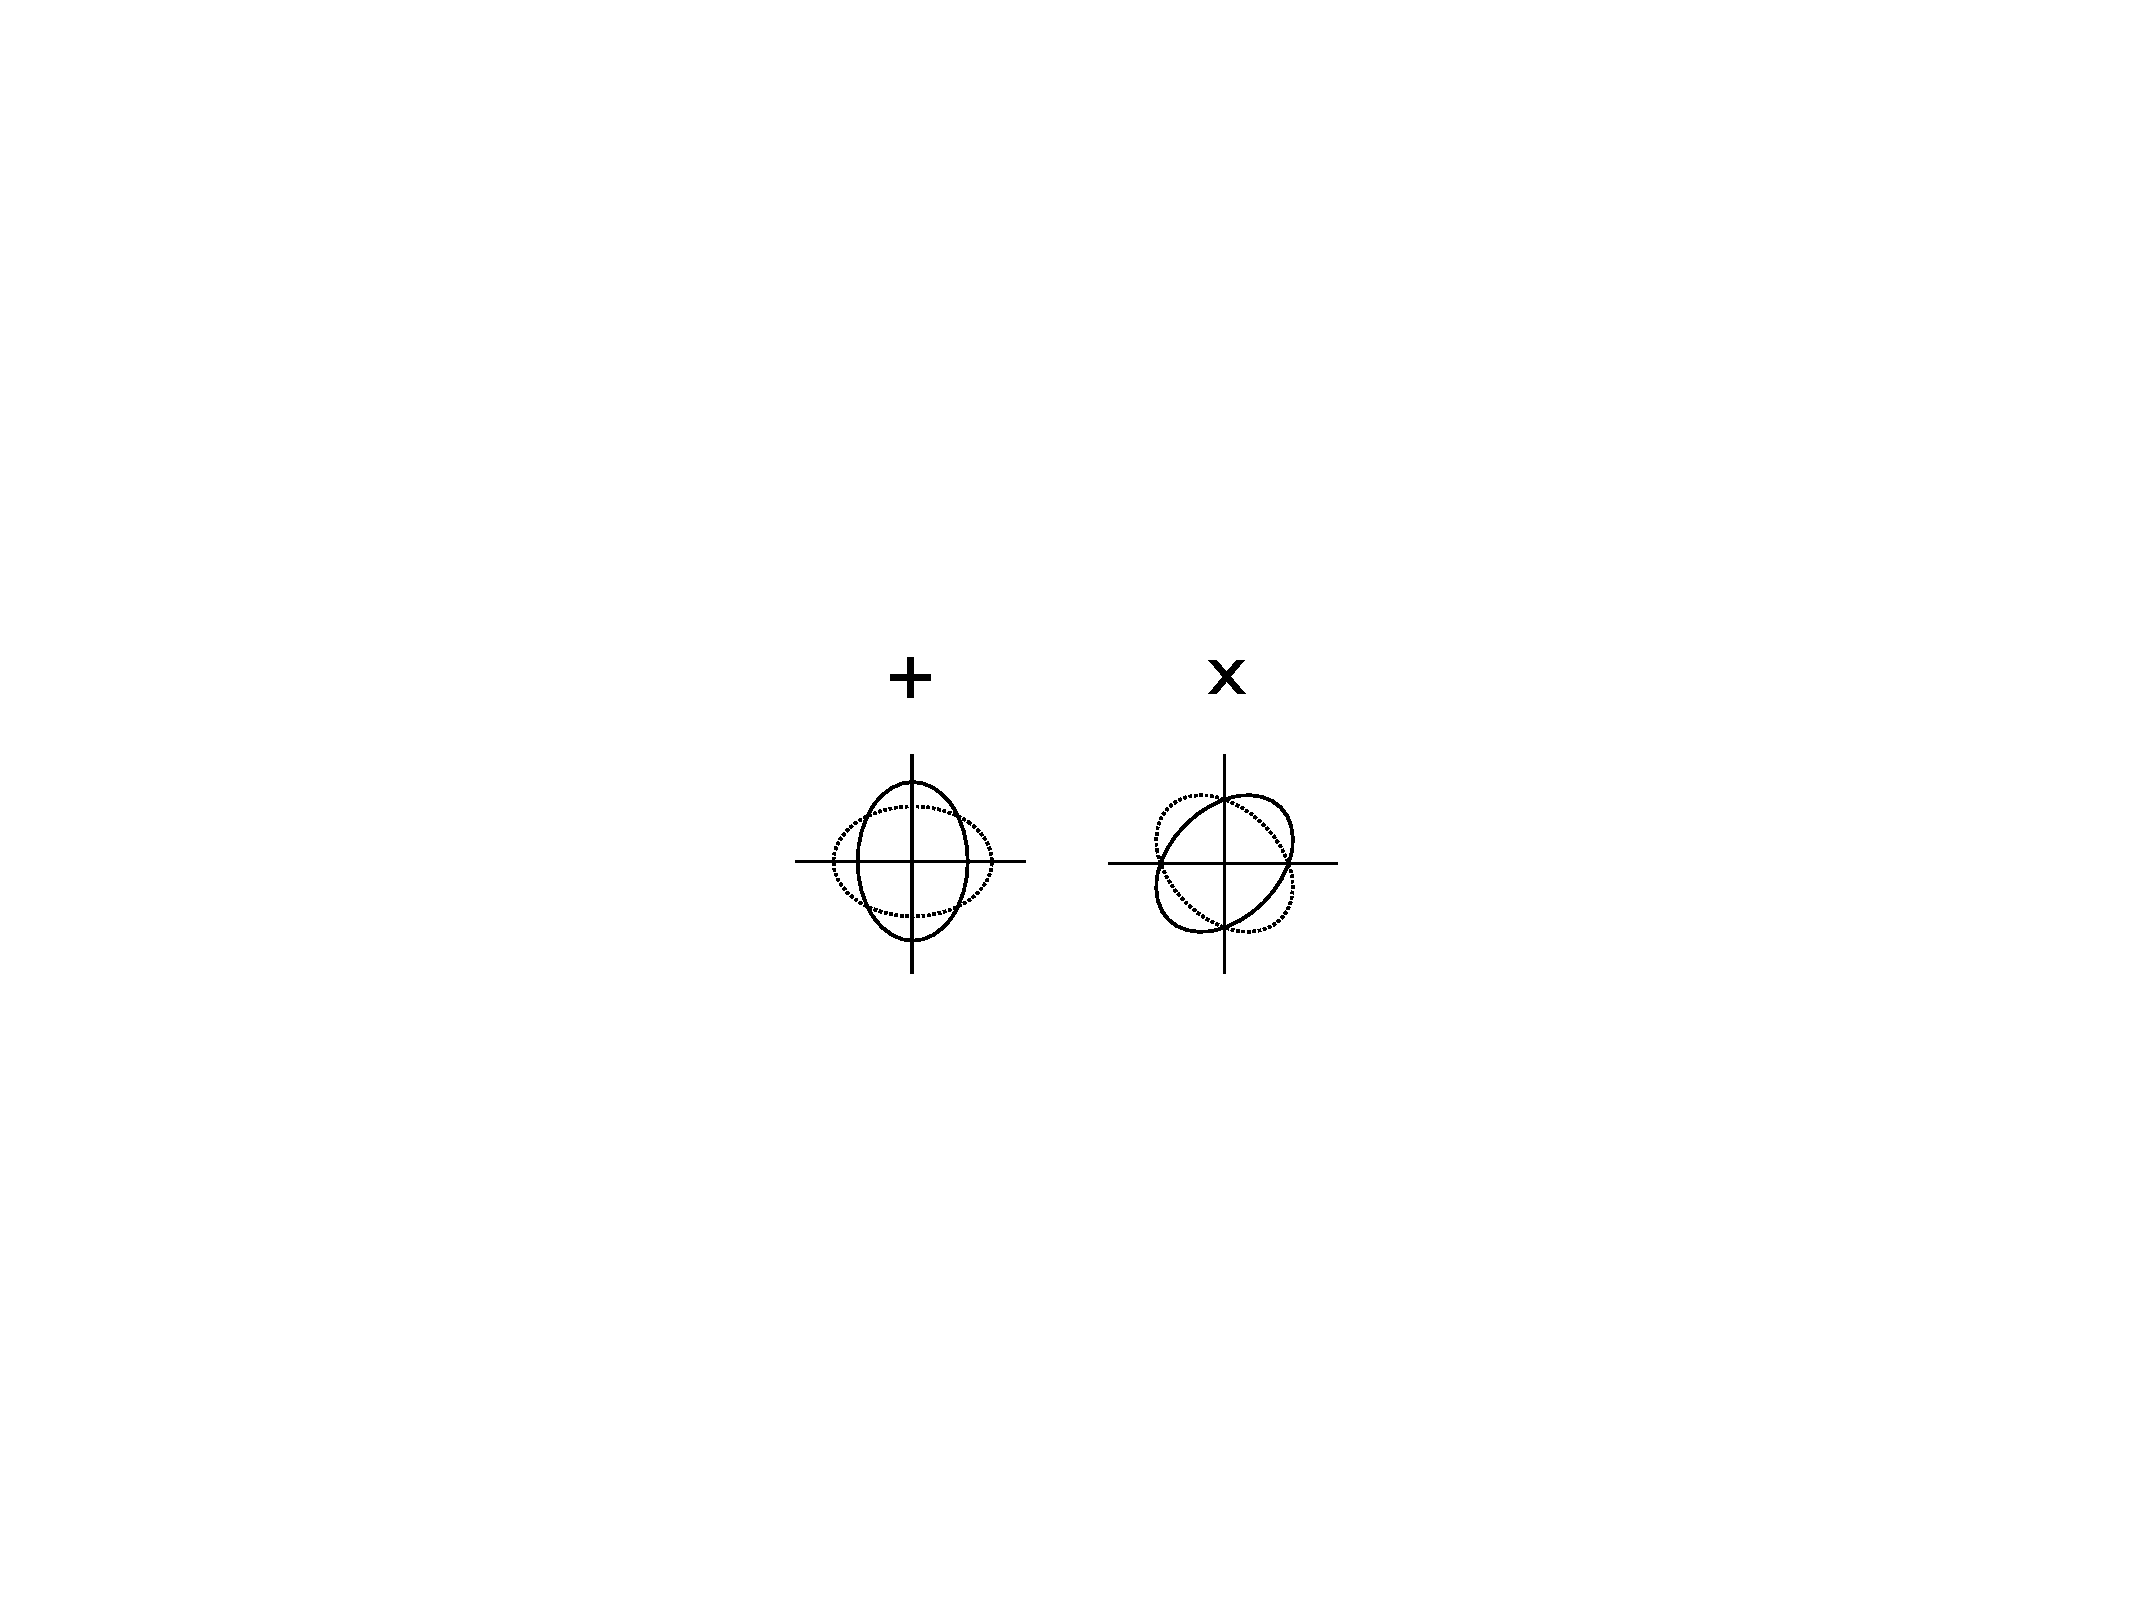
\includegraphics[width=0.4\textwidth]{Figures/polarizations}
\caption{The two orthogonal polarizations of a gravitational wave.
A circular ring of test particles in the plane orthogonal to 
the direction of propagation of the wave are alternately deformed
into ellipses, as space is ``squeezed" and ``stretched" by the 
passing of the wave.}
\label{f:polarizations}
\end{center}
\end{figure}
%
The metric perturbation for the most general GWB 
can thus be written as a superposition of such 
waves:
%
\be
h_{ab}(t,\vec x) =
\int_{-\infty}^\infty \D f\>
\int \D^2\Omega_{\hat k}\>
\sum_{A=+,\times}
h_A(f,\hat k)e^A_{ab}(\hat k) 
e^{i2\pi f(t-\hat k\cdot \vec x/c)}\,,
\label{e:planewave}
\ee
%
where $f$ denotes the frequency of the 
component waves, $\hat k$ their direction of
propagation, and $A=+,\times$ their polarization.
(The direction to a particular GW source is given 
by $\hat n=-\hat k$.)
%
\begin{figure}[htbp!]
\begin{center}
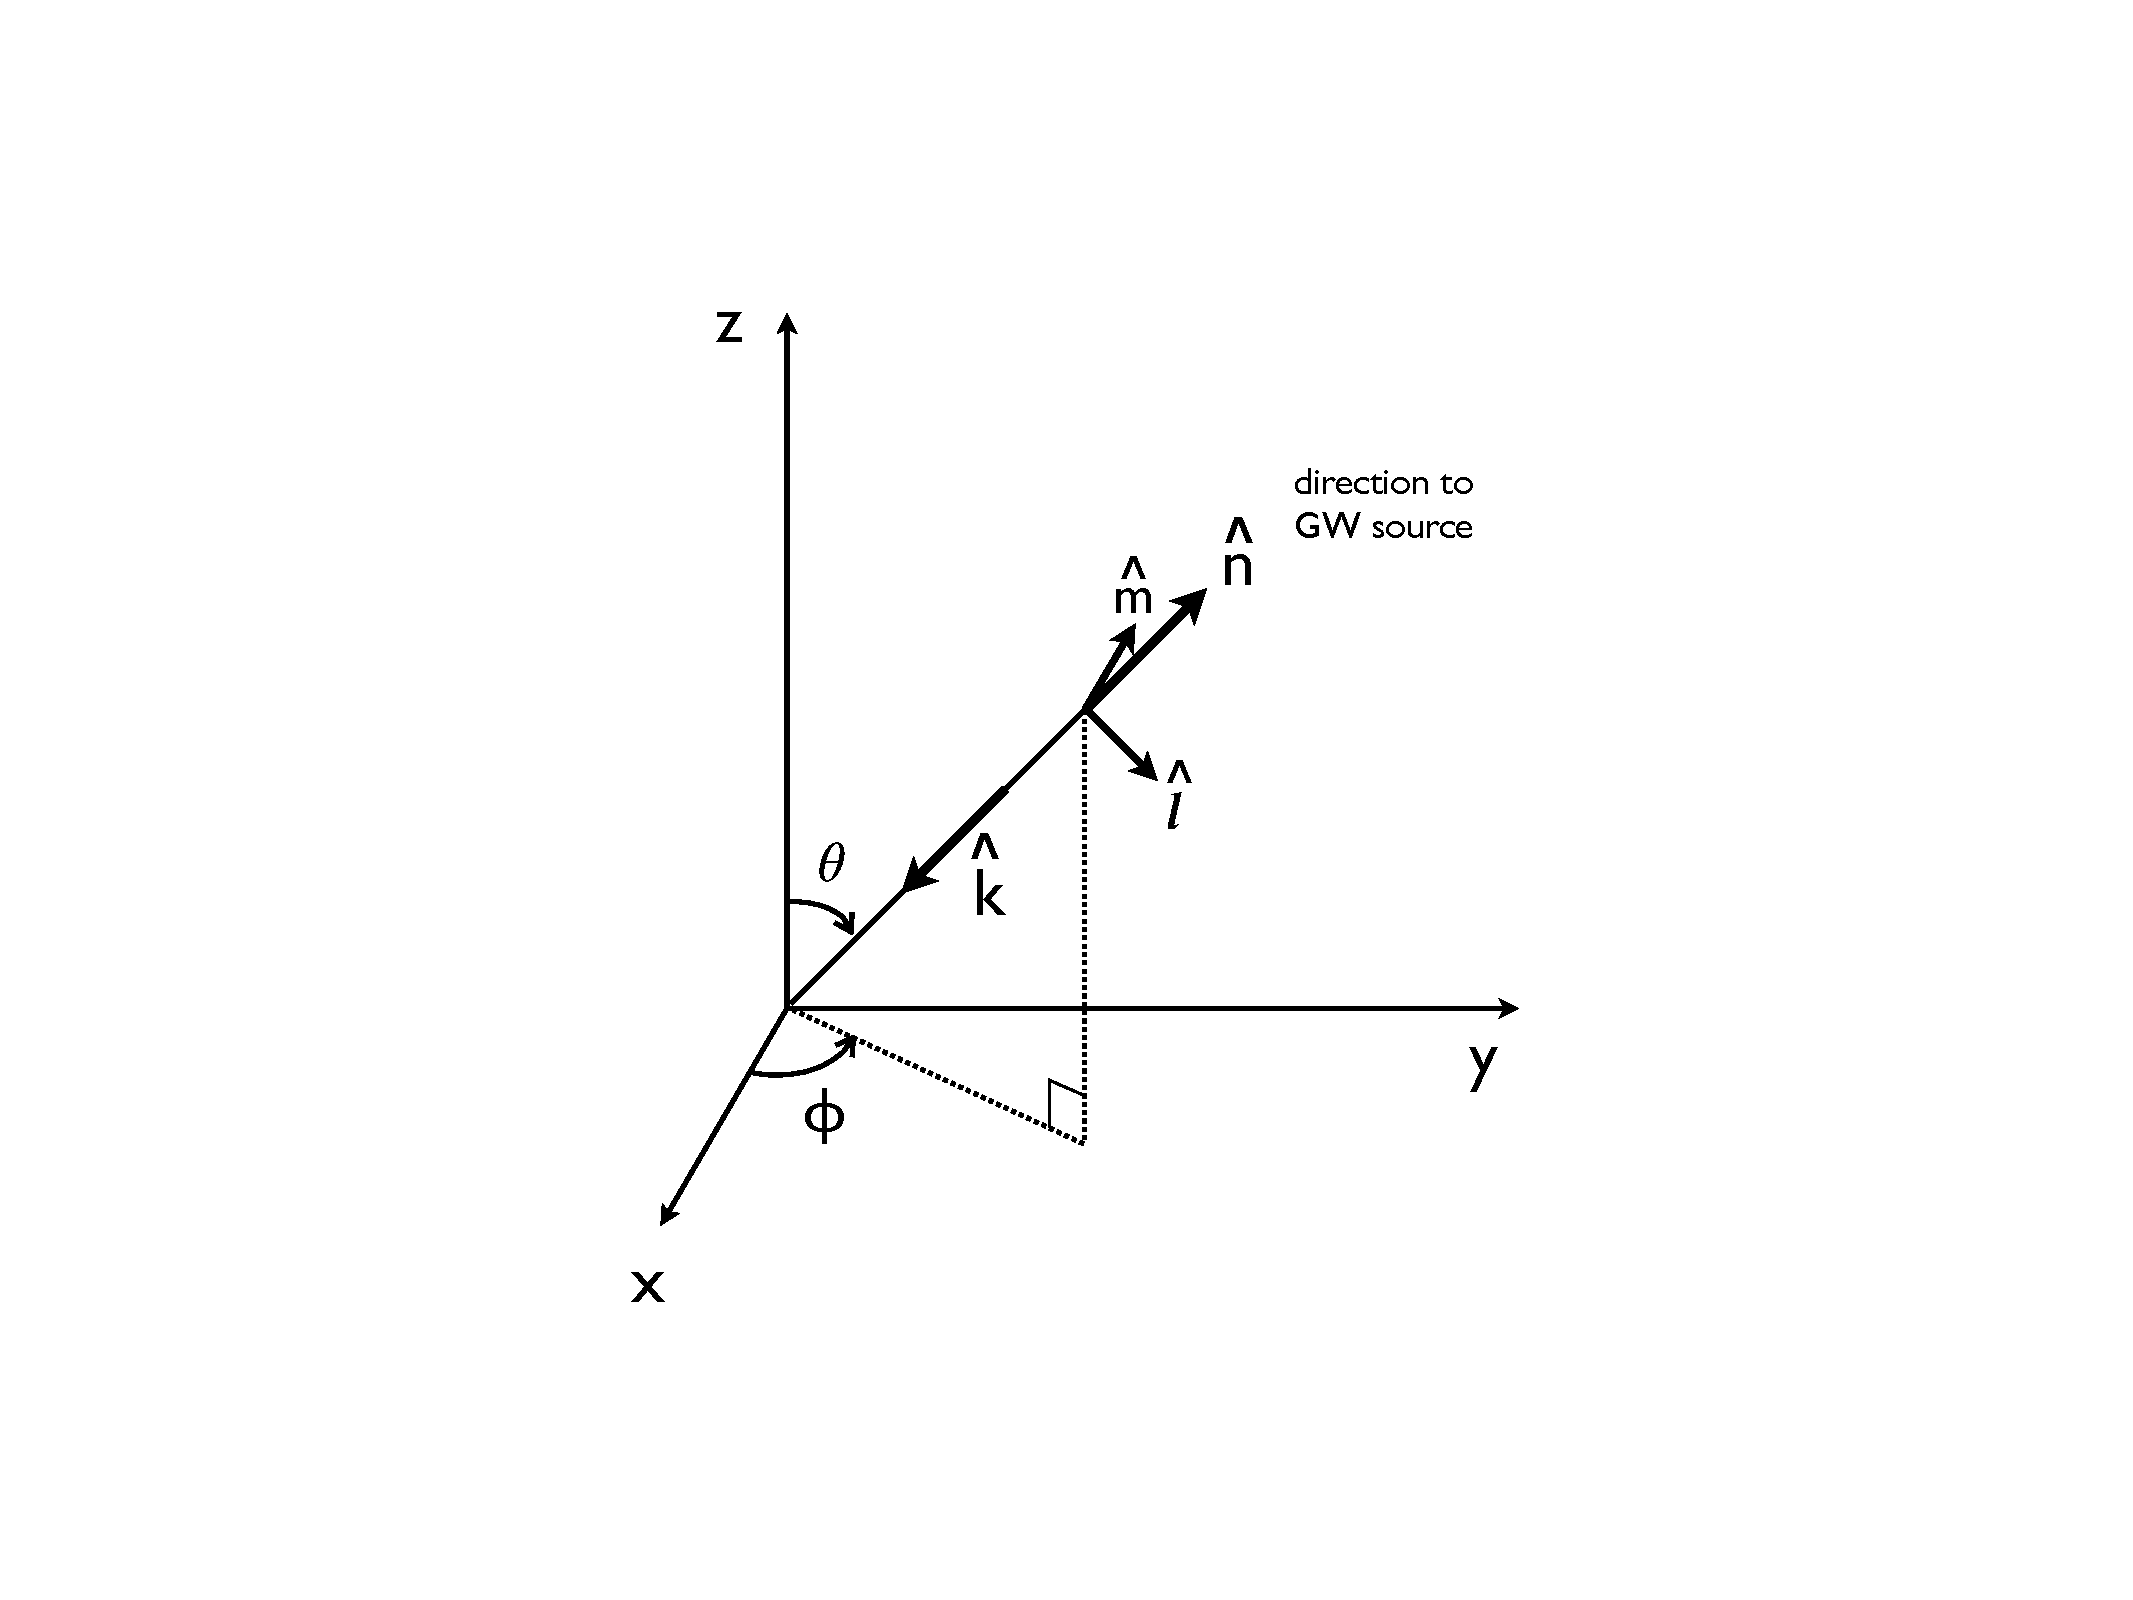
\includegraphics[width=0.4\textwidth]{Figures/plane_wave}
\caption{Coordinate system and unit vectors used in the 
plane-wave expansion of a GWB.}
\label{f:plane_wave}
\end{center}
\end{figure}
%
The quantities $e^A_{ab}(\hat k)$ are polarization
tensors, given by
%
\be
\begin{aligned}
e_{ab}^+(\hat k)
&=\hat l_a\hat l_b-\hat m_a\hat m_b\,,
\\
e_{ab}^\times(\hat k)
&=\hat l_a\hat m_b+\hat m_a\hat l_b\,,
\end{aligned}
\ee
%
where $\hat l$, $\hat m$ are any two orthogonal unit 
vectors in the plane orthogonal to $\hat k$.
Typically, for stochastic background analyses, 
we take $\hat l$, $\hat m$ to be proportional to 
the standard angular unit vectors tangent to the sphere,
so that $\{\hat k, \hat l, \hat m\}$ is a right-handed
system (Figure~\ref{f:plane_wave}):
%
\be
\begin{aligned}
\hat k
&=-\sin\theta\cos\phi\,\hat x
-\sin\theta\sin\phi\,\hat y
-\cos\theta\,\hat z
= -\hat r\,,
\\
\hat l
&=+\sin\phi\,\hat x
-\cos\phi\,\hat y
= -\hat\phi\,,
\\
\hat m
&=-\cos\theta\cos\phi\,\hat x
-\cos\theta\sin\phi\,\hat y
+\sin\theta\,\hat z 
= -\hat\theta\,.
\end{aligned}
\label{e:klm_def}
\ee
%
For analyzing non-stochastic GW sources that have 
a symmetry axis (e.g., the angular momentum 
vector for binary inspiral), one takes 
$\hat l$ and $\hat m$ to be rotated relative 
to $-\hat\phi$ and $-\hat\theta$, 
where the rotation angle is the 
{\em polarization angle} of the source.

\subsection{Ensemble averages}
\label{s:ensemble_averages}

The quantities $h_A(f,\hat k)$ are the Fourier 
coefficients of the plane wave expansion.
Since the metric perturbations 
for a stochastic background are random variables, 
so too are the 
Fourier coefficients.
The probability distributions of the Fourier coefficients
thus define the statistical properties of the background.

Without loss of generality, we can assume that the 
expected value of the Fourier coefficients is 
zero,
%
\be
\langle h_A(f,\hat k)\rangle=0\,,
\ee
%
where angle brackets denote {\em ensemble average}
over different realizations of the background.
(The different realizations could be thought of 
as the different backgrounds observed by
different spatially-located observers in a homogeneous 
and isotropic universe.)
The second-order moments (i.e., quadratic expectation 
values) specify possible correlations between the 
Fourier coefficients.
For example, if the background is 
{\em unpolarized, stationary, and isotropic}, then
%
\be
\langle h_A(f,\hat k)h_{A'}^*(f',\hat k')\rangle
=\frac{1}{16\pi} S_h(f)\delta(f-f')\delta_{AA'}\delta^2(\hat k,\hat k')\,,
\label{e:quad_iso}
\ee
%
where $S_h(f)$ is the {\em strain power spectral 
density} of the background, 
having units of ${\rm strain}^2\,{\rm Hz}^{-1}$.
The fact that the RHS is proportional 
to $\delta(f-f')$ is a consequence of the assumption
of {\em stationarity}---i.e., that there is no 
preferred origin of time.
That the RHS depends on the polarization indices
only via  $\delta_{AA'}$ is a consequence of the 
background being unpolarized---i.e., that the 
$+$ and $\times$ polarization components are statistically
equivalent and uncorrelated with one another.
Similarly, the dependence on GW propagation directions 
only via $\delta(\hat k,\hat k')$ is a consequence of 
exact isotropy,
i.e., that the power in the GWB has no preferred
direction, and that the GWs propagating in
different directions have uncorrelated phases.

If we drop the last assumption, allowing the background
to be either {\em anisotropic} or {\em statistically 
isotropic}, then the quadratic expectation values become
%
\be
\langle h_A(f,\hat k)h_{A'}^*(f',\hat k')\rangle
=\frac{1}{4} {\cal P}(f,\hat k)\delta(f-f')\delta_{AA'}
\delta^2(\hat k,\hat k')\,,
\label{e:quad_aniso}
\ee
%
where
%
\be
S_h(f) = \int \D^2\Omega_{\hat k}\,{\cal P}(f,\hat k)\,.
\ee
%
Here ${\cal P}(f,\hat k)$ is the strain power
spectral density per unit solid angle, with 
units ${\rm strain}^2\,{\rm Hz}^{-1}\,{\rm sr}^{-1}$.
For statistically isotropic backgrounds, the angular power 
spectra $C_l$ are the coefficients of a Legendre 
series expansion (\ref{e:legendre_series})
of the two-point function 
$C(\theta)\equiv 
\langle {\cal P}(f,\hat k){\cal P}(f,\hat k')\rangle_{\rm sky\ avg}$, 
for all $\hat k$, $\hat k'$ having 
$\cos\theta = \hat k\cdot \hat k'$.

For {\em Gaussian} backgrounds, all cubic 
and higher-order moments are either identically zero 
or can be written in terms of the second-order moments.
Thus, the quadratic expectation values of the Fourier
coefficients completely characterize the statistical
properties of a Gaussian-distributed background.

\subsection{Energy density spectrum in gravitational waves}
\label{s:Omega_gw}

As mentioned above, $S_h(f)$ is the strain power 
spectral density of the GWB.
It can be related to the (normalized) 
{\em energy density spectrum}
%
\be
\Omega_{\rm gw}(f) 
\equiv \frac{1}{\rho_{\rm c}}\frac{\D\rho_{\rm gw}}{\D\ln f}
=\frac{f}{\rho_{\rm c}}\frac{\D\rho_{\rm gw}}{\D f}\,,
\label{e:Omega_gw}
\ee
%
where $\D\rho_{\rm gw}$ is the energy density in gravitational
waves contained in the frequency interval $f$ to $f+\D f$, and 
$\rho_{\rm c}\equiv {3 H_0^2 c^2}/{8\pi G}$
is the {\em critical} energy density (that needed to just 
close the universe today).
The result is 
%
\be
S_h(f) = \frac{3H_0^2}{2\pi^2}\frac{\Omega_{\rm gw}(f)}{f^3}\,,
\label{e:S_h_and_Omega_gw}
\ee
%
which makes use of the relation
%
\be
\rho_{\rm gw} = \frac{c^2}{32\pi G}
\langle \dot h_{ab}(t,\vec x)\dot h^{ab}(t,\vec x)\rangle\,,
\label{e:rho_gw}
\ee
%
which gives the energy density in gravitational waves
in terms of the quadratic expectation values of the
metric perturbations.
You are asked in Exercise~\ref{exer:2} to derive
(\ref{e:S_h_and_Omega_gw}); to do so, 
you will also need to use the 
plane-wave expansion (\ref{e:planewave})
and the quadratic expectation values 
\eqref{e:quad_iso} or \eqref{e:quad_aniso}.

In addition to $S_h(f)$ and $\Omega_{\rm gw}(f)$, one
sometimes describes the strength of a GWB in terms of
the (dimensionless) {\em characteristic strain}
$h_c(f)$ defined by
%
\be
h_c(f) = \sqrt{f S_h(f)}\,.
\ee
%
For backgrounds described by a power-law dependence
on frequency,% 
\footnote{There is no sum over $\alpha$ or $\beta$ in 
the following expressions.}
%
\be
h_c(f) = A_\alpha \left(\frac{f}{f_{\rm ref}}\right)^\alpha\,
\quad\Leftrightarrow\quad
\Omega_{\rm gw}(f) = \Omega_\beta\left(\frac{f}{f_{\rm ref}}\right)^\beta\,,
\label{e:powerlaw}
\ee
%
where $\alpha$ and $\beta$ are spectral indices,
and $A_\alpha$ and $\Omega_\beta$ are the amplitudes 
of the characteristic strain and energy density 
spectrum, respectively, at some reference frequency
$f=f_{\rm ref}$.
Using the above definitions and relationships between
$\Omega_{\rm gw}(f)$, $S_h(f)$, and $h_c(f)$, we have
%
\be
\Omega_\beta = \frac{2\pi^2}{3 H_0^2}f_{\rm ref}^2 A_\alpha^2\,,
\qquad
\beta = 2\alpha +2\,.
\ee
%
For standard inflationary backgrounds, $\Omega_{\rm gw}(f)={\rm const}$,
for which $\beta=0$ and $\alpha=-1$.
For GWBs associated with binary inspiral, 
$\Omega_{\rm gw}(f)\propto f^{2/3}$ (as we shall show below),
for which $\beta=2/3$ and $\alpha=-2/3$.
This last dependence is valid for both compact binary coalescences 
consisting of NSs and/or 
stellar-mass BHs (relevant for advanced LIGO, Virgo, etc.),
and also for inspirals of SMBHs
in the centers of distant galaxies (relevant for pulsar timing searches).
 
\subsection{Calculating $\Omega_{\rm gw}(f)$ for an
astrophysically-generated background}
\label{s:Phinney_formula}

There is a relatively simple formula for calculating
the energy density spectrum $\Omega_{\rm gw}(f)$ 
produced by a collection of discrete astrophysical GW 
sources distributed throughout the universe\cite{Phinney:2001}:
%
\be
\left.
\Omega_{\rm gw}(f) = \frac{1}{\rho_{\rm c}}\int_0^\infty \D z\>
n(z) \frac{1}{1+z}\left(f_{\rm s}\frac{\D E_{\rm gw}}{\D f_{\rm s}}
\right)\right|_{f_{\rm s}=f(1+z)}\,.
\label{e:phinney1}
\ee
%
We will call this the ``Phinney formula", since it was 
first written down by E.S.~Phinney in an unpublished
paper in 2001.
For this expression,
one needs only the comoving number density of
sources $n(z)$ as a function of the cosmological redshift $z$, 
and the energy spectrum of an individual source
$\D E_{\rm gw}/\D f_s$ as measured in its rest frame.
The source frame frequency $f_{\rm s}$ is related to the 
observed (present-day) frequency $f$ via $f_{\rm s}=f(1+z)$.
The factor of $1/(1+z)$ in the integrand is needed to 
redshift the energy measured in the source frame to that
measured today.

The above relationship can also be written in terms of 
the comoving rate density $R(z)$, which is related to the
comoving number density $n(z)$ via
%
\be
n(z)\,\D z = R(z)\,|\D t|_{t=t(z)}\,.
\ee
%
The result is
%
\be
\left.
\Omega_{\rm gw}(f) = \frac{f}{\rho_{\rm c}H_0}\int_0^\infty \D z\>
R(z) \frac{1}{(1+z)E(z)}\left(\frac{\D E_{\rm gw}}{\D f_{\rm s}}
\right)\right|_{f_{\rm s}=f(1+z)}\,,
\label{e:phinney2}
\ee
%
where 
%
\be
E(z)\equiv \sqrt{\Omega_{\rm m}(1+z)^3 + \Omega_\Lambda}
\ee
%
is a cosmological factor that arises when evaluating $\D t/\D z$.
$\Omega_{\rm m}$ and $\Omega_\Lambda$ are the 
fractional energy densities for matter
(ordinary baryonic matter plus dark matter) 
and dark energy, with numerical values roughly
equal to $0.30$ and $0.70$, respectively.
Exercise~\ref{exer:3} asks you to prove this 
``rate-version" of the Phinney formula, filling in some 
of the cosmology-related details.

\subsubsection{Example: $\Omega_{\rm gw}(f)$ for binary inspiral}
\label{s:binary_inspiral}

To illustrate the Phinney formula in action, we will 
verify the $\Omega_{\rm gw}(f)\propto f^{2/3}$
power-law dependence for binary inspiral, which we
stated without proof at the end of Section~\ref{s:Omega_gw}.
Since we are interested here only in the frequency 
dependence of $\Omega_{\rm gw}(f)$, all we need to 
calculate is the energy spectrum $\D E_{\rm gw}/\D f_{\rm s}$
for a single binary system.

So let us consider two masses, $m_1$ and $m_2$, in circular 
orbits around their common center of mass (Figure~\ref{f:binary_inspiral}).
%
\begin{figure}[htbp!]
\begin{center}
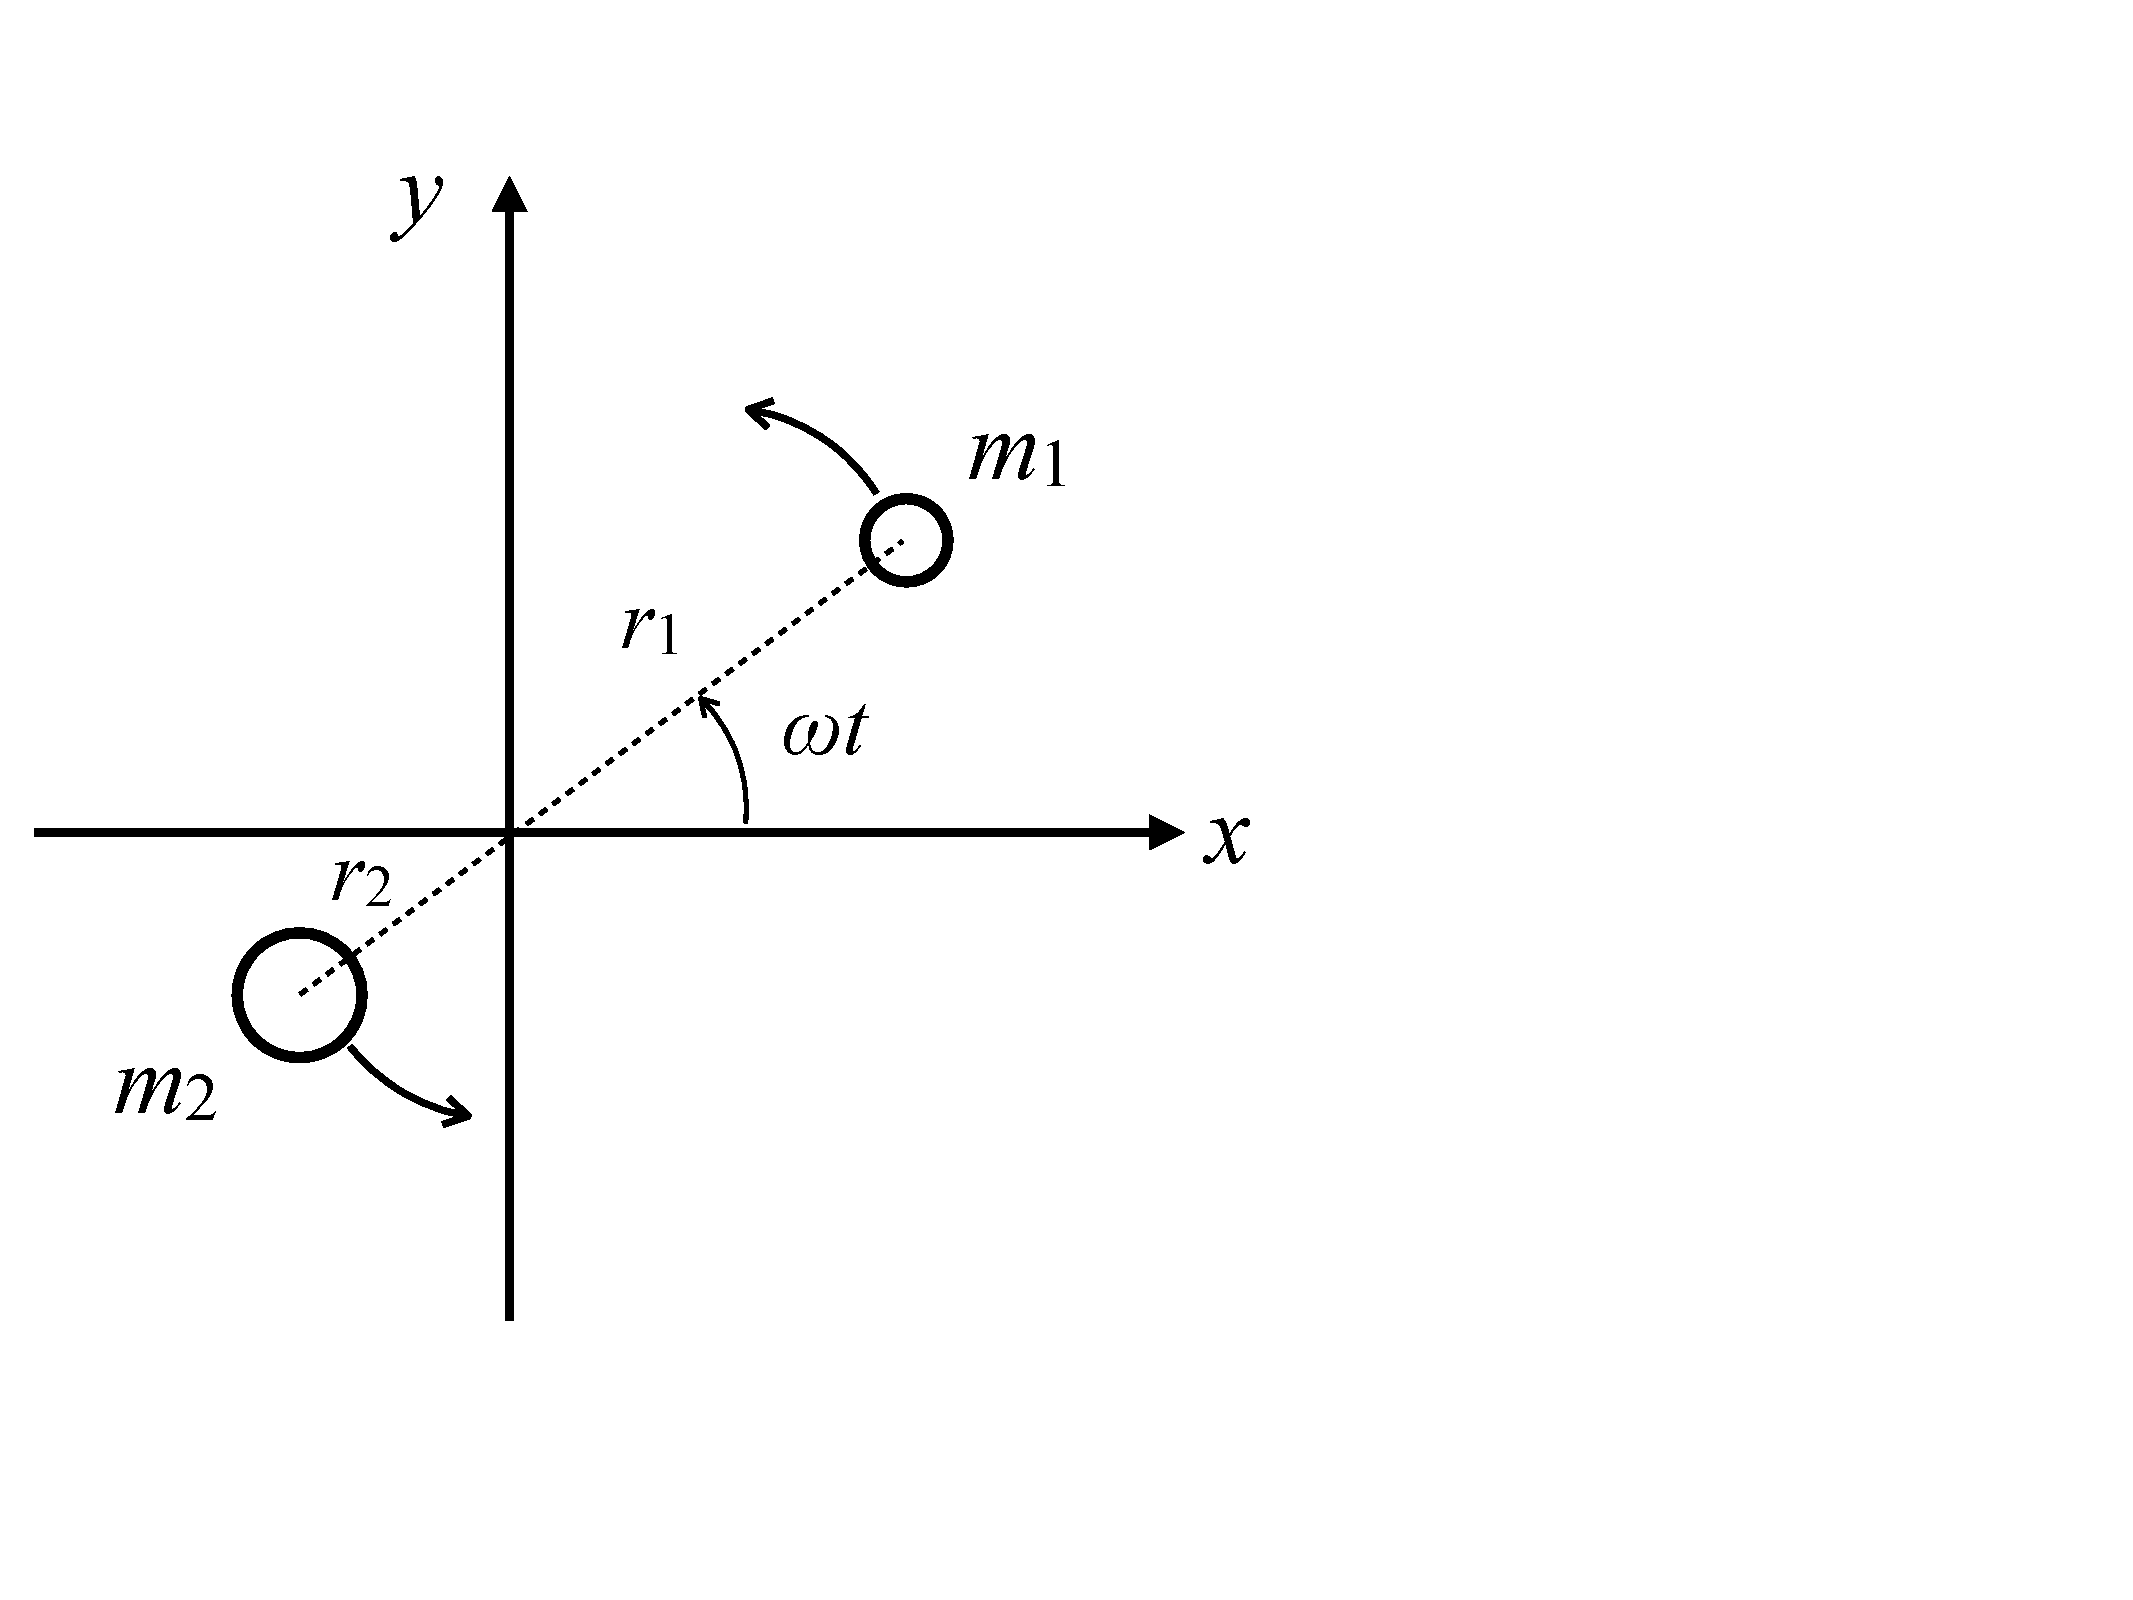
\includegraphics[width=0.4\textwidth]{Figures/binary_inspiral}
\caption{Two masses $m_1$, $m_2$ in orbit around their common
of mass.}
\label{f:binary_inspiral}
\end{center}
\end{figure}
%
We make the standard definitions
%
\be
\begin{aligned}
r\equiv r_1+r_2\,,\quad
M\equiv m_1 + m_2\,,\quad
\mu\equiv \frac{m_1 m_2}{m_1 + m_2}
\end{aligned}
\ee
%
of the {\em relative separation}, {\em total mass}, 
and {\em reduced mass} of the system.
In terms of these quantities, Kepler's third law and 
the total orbital energy of the system can be written as
\be
\omega^2 r^3 = GM\,,\qquad
E_{\rm orb} = -\frac{GM\mu}{2r}\,,
\ee
%
where $\omega\equiv 2\pi f_{\rm orb}$ is the orbital 
angular frequency.
The power emitted in gravitational waves comes from
the orbital energy
%
\be
\frac{\D E_{\rm gw}}{\D t} 
= -\frac{\D E_{\rm orb}}{\D t}\,,
\ee
%
which implies that the energy spectrum is given by
%
\be
\frac{\D E_{\rm gw}}{\D f_{\rm s}} 
= \frac{\D t}{\D f_{\rm s}}\frac{\D E_{\rm gw}}{\D t}
= -\frac{\D t}{\D f_{\rm s}}\frac{\D E_{\rm orb}}{\D t}\,.
\ee
%
It is now a relatively simple matter to evaluate the
RHS of the last expression, using Kepler's law to 
replace all occurences of $r$ and $\dot r$ with 
expressions involving $\omega$ and $\dot\omega$.
The final result is 
%
\be
\frac{\D E_{\rm gw}}{\D f_{\rm s}} 
\sim {\cal M}_{\rm c}^{5/3} f_{\rm s}^{-1/3}\,,
\qquad
{\cal M}_c^{5/3} \equiv M^{2/3}\mu\,,
\ee
%
where ${\cal M}_{\rm c}$ is the {\em chirp mass} of 
the system, and where we have ignored all numerical
factors.
Note that we also replaced the orbital angular frequency
$\omega$ by the GW frequency
$f_{\rm s} = 2 f_{\rm orb}$, with the factor of 2 
arising for quadrupolar radiation in general relativity.%
\footnote{For elliptical orbits, one should average
the radiated power, etc., over a period of the orbit.
There will also be contributions to the gravitational
radiation from harmonics other than just the quadrupole.} 
Returning now to (\ref{e:phinney2}), we substitute
$f_s=(1+z)f$ and multiply by the factor of $f$ outside 
the integral to get
$\Omega_{\rm gw}(f) \propto f^{2/3}$ as claimed.

%%%%%%%%%%%%%%%%%%%%%%%%%%%%%%%%%%%%%%%%%%%%%%%%%%%%%%%
\section{Correlation methods}
\label{s:correlations}

As discussed above, a stochastic background of GWs 
is described by a {\em random} signal, which looks 
like noise in a single detector.
As such, standard search techniques like 
{\em matched filtering}, which correlate the data 
against known, deterministic waveforms (e.g., BBH chirps) 
won't work when trying to detect a GWB.
Instead, we have to consider other possibilities:
(i) One possibility is to know the noise sources 
in our GW detector well enough (in both 
amplitude and spectral shape) that we can 
attribute any unexpected excess ``noise" to a GWB.
(This was basically how Penzias and Wilson 
initially detected the CMB; they saw an excess 
noise temperature of $\sim\!3.5^\circ~{\rm K}$ in their
radio antenna that they could not attribute to 
any other noise source.)
(ii) Another possibility is to use data from 
multiple detectors.
Then we can look for evidence of a common 
disturbance in the multiple data streams 
consistent with each detector's response to 
gravitational waves.

Currently, (i) is not an option for ground-based 
interferometers since, even though the individual 
noise sources 
are understood pretty well, their amplitude is not 
known precisely enough to attribute any observed 
excess power to gravitational waves.
One would need a really loud GWB relative to the
detector noise in order detect it in a way similar
to Penzias and Wilson's detection of the CMB.
But (ii) is an option as LIGO consists of two 
detectors, one in Hanford, WA, the other in Livingston, LA.
Virgo, in Italy, provides a third detector, 
and soon we will have two more large-scale 
interferometers in Japan and India.
Cross-correlating data from multiple detectors works
for detecting a GWB since, even though the signal is 
random, it is the {\em same} signal in the different 
dectors (modulo the physical separation and relative
orientation of the detectors).
In effect, the random output of one detector is
used as a template for the data in another detector.
As we shall see below, the signal-to-noise ratio of 
the cross-correlation grows like the square-root of 
the observation time.
Thus, although the GWB might be weak 
relative to the noise, it can still be extracted from 
a cross-correlation measurement if it is observed
for a long enough period of time.

\subsection{Basic idea}
\label{s:basic_idea}

To illustrate the basic idea behind cross-correlation,
we will consider first the simplest possible scenario---i..e,
a single sample of data from two colocated and coaligned
detectors:
%
\be
\begin{aligned}
d_1 &= h + n_1\,,
\\
d_2 &= h + n_2\,.
\end{aligned}
\ee
%
Here $h$ denotes the common GW signal component, 
and $n_1$, $n_2$ denote the corresponding instrumental
noise components.
Cross-correlating the data for this case amounts to 
simply taking the product of the two data 
samples, $\hat C_{12}\equiv d_1 d_2$.
The expected value of the cross-correlation is
%
\be
\langle \hat C_{12}\rangle
=\langle d_1 d_2\rangle
= \langle h^2\rangle + \cancelto{0}{\langle h n_2\rangle} 
+ \cancelto{0}{\langle n_1 h\rangle}
+ \langle n_1 n_2\rangle\,,
\ee
%
where $\langle h n_2\rangle = 0 = \langle n_1 h\rangle$,
since the GW signal and instrumental noise are not correlated
with one another.
If we further assume that the noise in the two detectors
is {\em uncorrelated} (which is a good valid assumption 
if the detectors are widely separated%
\footnote{Note that global magnetic fields, e.g., Schumann 
resonances, {\em can} produce environmental correlations in 
widely separated detectors.}), then $\langle n_1 n_2\rangle =0$,
leaving
%
\be
\langle \hat C_{12}\rangle = \langle h^2\rangle\equiv S_h\,,
\ee
which is just the variance (i.e., power) in the GW signal.

\subsection{Extension to multiple data samples}
\label{s:multiple_samples}

The above analysis can be easily extended to the case of 
multiple samples:
%
\be
\begin{aligned}
d_{1i} &= h_i + n_{1i}\,,
\\
d_{2i} &= h_i + n_{2i}\,,
\end{aligned}
\ee
%
where $i=1,2,\cdots,N$.
As before, we will assume that the two detectors are
coincident and coaligned, and that the noise in the
two detectors are uncorrelated with the GW signal 
and with one another
%
\be
\langle n_{1i} h_j\rangle = 0\,,
\qquad
\langle n_{2i} h_j\rangle = 0\,,
\qquad
\langle n_{1i}n_{2j}\rangle=0\,.
\ee
%
We will also assume that the GWB 
and detector noise are both {\em white}, which means 
%
\be
\langle h_ih_j\rangle = S_h\,\delta_{ij}\,,
\qquad
\langle n_{1i}n_{1j}\rangle = S_{n_1}\,\delta_{ij}\,,
\qquad
\langle n_{2i}n_{2j}\rangle = S_{n_2}\,\delta_{ij}\,,
\ee
%
where $S_h$, $S_{n_1}$, $S_{n_2}$ are the variances
(i.e., power) in the GW signal and detector noise, respectively.%
\footnote{The assumption that both the GWB and detector noise
are white is made here just to simplify the analysis.
One can use cross-correlation methods for the more 
general case where the signal and noise power spectral
densities are non-trivial functions of frequency~\cite{allen-romano}.}
For this case, our cross-correlation statistic is the
average of the products of the individual data samples
%
\be
\hat S_h 
\equiv \hat C_{12} 
\equiv \frac{1}{N}\sum_{i=1}^N d_{1i} d_{2i}\,,
\ee
%
which, as we shall see below, is again an estimator of the 
power in the GWB (hence the ``hat" ($\hat{\ }$) over the 
$S_h$ on the LHS of this equation).

Using the above definitions and quadratic expectation 
values, it is easy to show that
%
\be
\mu\equiv \langle \hat C_{12}\rangle
= \frac{1}{N}\sum_{i=1}^N \langle d_{1i} d_{2i}\rangle
= \frac{1}{N}\sum_{i=1}^N \langle h_i^2\rangle
= S_h\,.
\ee
%
Thus, the cross-correlation statistic $\hat C_{12}$ is 
an (unbiased) estimator of the GW power $S_h$.
The variance in this estimator can be calculated via
%
\be
\sigma^2\equiv \langle \hat C_{12}^2\rangle-
\langle \hat C_{12}\rangle^2
=\left(\frac{1}{N}\right)^2
\sum_{i=1}^N \sum_{j=1}^N 
\left(\langle d_{1i} d_{2i} d_{1j} d_{2j}\rangle - 
\langle d_{1i} d_{2i}\rangle \langle d_{1j} d_{2j}\rangle\right)\,.
\label{e:sigma2_def}
\ee
%
To evaluate the RHS of the above equation, we make use of 
the identity
%
\be
\langle abcd\rangle =
\langle ab\rangle\langle cd\rangle + \langle ac\rangle \langle bd\rangle 
+\langle ad\rangle \langle bc\rangle\,,
\ee
%
which is valid for zero-mean Gaussian random variables.
Using this identity and the quadratic expectation values
between the signal and noise, we end up with
%
\be
\sigma^2 = \frac{1}{N}(S_1 S_2 + S_h^2)\,,
\label{e:sigma2_final}
\ee
%
where 
%
\be
S_1\equiv S_{n_1} + S_h\,,
\qquad
S_2\equiv S_{n_2} + S_h\,,
\ee
%
are the total power in the detector output (consisting of 
both signal and noise power).
Note that the factor of $1/N$ in \eqref{e:sigma2_final} 
comes from the double sum in \eqref{e:sigma2_def} having
non-zero contributions from only the diagonal terms $(i=j)$, 
which are all equal to one another.

Since the power in the GWB is expected to be weak compared
to the detector noise, the variance can be approximated
as $\sigma^2\simeq S_1 S_2/N$, for which the expected 
signal-to-noise ratio is given by
%
\be
\rho\equiv \frac{\mu}{\sigma}\simeq \frac{S_h}{\sqrt{S_1 S_2/N}}
\simeq \sqrt{N}\,\frac{S_h}{S_n}\,,
\ee
%
where $\sqrt{S_1 S_2}\simeq\sqrt{S_{n_1} S_{n_2}}\equiv S_n$.
This result verifies the statement made earlier that the signal-to-noise
ratio for a cross-correlation measurement grows like the square-root 
of the observation time (in this case, the total number of samples).

\subsection{Optimal filtering}
\label{s:optimal_filtering}

To handle the case of physically-separated and misaligned 
detectors, we need to include the non-trivial response of 
a GW detector to a GWB.  
We will do this in more detail in 
Sections~\ref{s:nontrivial_response} and
\ref{s:nontrivial_correlations}.
Here, it suffices to simply define the {\em overlap function} 
(or overlap reduction function),
denoted $\Gamma_{12}(f)$, as the transfer function relating
the strain power in the GWB, $S_h(f)$, 
to the cross-correlated signal power 
in the two detectors, 
%
\be
C_{12}(f) \equiv \Gamma_{12}(f) S_h(f)\,.
\ee
%
(We will derive the form of $\Gamma_{12}(f)$ and discuss
more of its properties in Section~\ref{s:nontrivial_correlations}.)
In terms of the quadratic expectation values of the GW 
signal in the two detectors, we have%
\footnote{The factor of $1/2$ is included on the RHS
so that the power spectrum is {\em one-sided}.
In other words, 
the total cross-correlated power in the GWB is
given by the integral of $\Gamma_{12}(f)S_h(f)$ over just
the {\em positive} frequencies.
The factor of $\delta(f-f')$ is a consequence of stationarity.}:
%
\be
\langle \tilde h_1(f) \tilde h_2^*(f')\rangle
=\frac{1}{2}\delta(f-f')\Gamma_{12}(f)S_h(f)\,,
\ee
%
where $\tilde h_1(f)$, $\tilde h_2(f)$ denote the 
Fourier transforms of GW signal components 
$h_1(t)$, $h_2(t)$ in  the two detectors.
For comparison, the (auto-correlated) power spectra 
of the detector noise $P_{n_1}(f)$, $P_{n_2}(f)$ 
can be written in terms of the noise components 
$\tilde n_1(f)$, $\tilde n_2(f)$ via:
%
\be
\begin{aligned}
\label{e:noise_power_spectra}
\langle \tilde n_1(f) \tilde n_1^*(f')\rangle
&=\frac{1}{2}\delta(f-f')P_{n_1}(f)\,,
\\
\langle \tilde n_2(f) \tilde n_2^*(f')\rangle
&=\frac{1}{2}\delta(f-f')P_{n_2}(f)\,,
\end{aligned}
\ee
%
while the cross-correlated noise is assumed to be zero:
%
\be
\langle \tilde n_1(f) \tilde n_2^*(f')\rangle =0\,.
\ee
Plots of $\Gamma_{12}(f)$ for the 
LIGO Hanford-LIGO Livingston interferometer pair 
and for the LIGO Hanford-Virgo interferometer pair 
can be found in 
Section~\ref{s:nontrivial_correlations}.

Given the above definitions, we can now ask
the question: ``What is the optimal way to correlate 
data from two physically separated and possibly 
mis-aligned detectors to search for a GWB?"
To answer this question, we start by forming the 
generic cross-correlation
%
\be
\hat C_{12} = \int_{-T/2}^{T/2}\D t\>\int_{-T/2}^{T/2}\D t'\>
d_1(t)d_2(t) Q(t,t')\,,
\ee
%
where $Q(t,t')$ is an a~apriori arbitrary filter 
function and $T$ is the observation time.
For stationary data, $Q(t,t')$ should depend only on
the difference between the two time arguments, 
$\Delta t\equiv t-t'$, 
so that $Q(t,t')\equiv Q(t-t')$.
In the Fourier domain, we can then write
%
\be
\hat C_{12} \simeq 
\int_{-\infty}^{\infty}\D f\>\int_{-\infty}^{\infty}\D f'\>
\delta_T(f,f')\tilde d_1(f)\tilde d_2(f') \tilde Q^*(f')\,,
\ee
%
where $\tilde Q(f)$ is the Fourier transform of 
$Q(\Delta t)$, and $\delta_T(f-f')$ is a finite-time
version of the Dirac delta function defined by 
$\delta_T(f-f')\equiv T\,{\rm sinc}\,(\pi(f-f'))$, where
${\rm sinc}\,x \equiv \sin x/x$.

To proceed further we need to define what we mean by 
{\em optimal}.
A natural criterion in this context is to maximize the 
expected signal-to-noise ratio of $\hat C_{12}$ 
for a GWB with a fixed spectral shape $H(f)$.
(The expected signal-to-noise ratio is defined as 
in the previous section
$\rho\equiv \mu/\sigma$, where 
$\mu\equiv\langle \hat C_{12}\rangle$
and 
$\sigma^2\equiv \langle \hat C_{12}^2\rangle -\langle
\hat C_{12}\rangle^2$.) 
As you are asked to show in Exercise~\ref{exer:4},
this maximization condition  determines the form of the 
filter 
function $\tilde Q(f)$ up to an overall normalization:
%
\be
\tilde Q(f) \propto \frac{\Gamma_{12}(f) H(f)}
{P_1(f) P_2(f)}\,,
\ee
%
where $P_1(f)$, $P_2(f)$ are the total power in the two
detectors, 
%
\be
\begin{aligned}
P_1(f) \equiv P_{n_1}(f) + P_h(f)\,,
\qquad
P_2(f) \equiv P_{n_2}(f) + P_h(f)\,,
\end{aligned}
\ee
%
which are approximately equal to 
$P_{n_1}(f)$, $P_{n_2}(f)$ under the assumption that 
the GW signal is weak compared to the detector noise.
Note that the numerator of $\tilde Q(f)$ is proportional
to the expected value of the cross-correlated data in
the frequency domain, 
$\langle \tilde d_1(f)\tilde d_2^*(f)\rangle$,
while the denominator basically de-weights the 
correlation when the detector noise is large.
The dependence of $\tilde Q(f)$ on the spectral shape
$H(f)$ means that the optimal filter is tuned to a 
particular GWB.

The overall normalization of the optimal filter $\tilde Q(f)$ 
is not determined by the maximation condition, since
a constant multiplicative factor cancels out when
calculating  the signal-to-noise ratio $\rho=\mu/\sigma$.  
Typically, we use this freedom in the choice of 
normalization to set the expected value $\mu$ of the
cross-correlation equal to the overall amplitude of 
the background---i.e., $\mu = \Omega_{\rm gw}(f_{\rm ref})$.
In other words, for this choice of normalization, 
the measured value of the 
cross-correlation statistic, $\hat C_{12}$, is a 
{\em point estimate} of $\Omega_{\rm gw}(f_{\rm ref})$.

%%%%%%%%%%%%%%%%%%%%%%%%%%%%%%%%%%%%%%%%%%%%%%%%%%%%%%%
\section{Optimal filtering applied to some simple examples}
\label{s:simple_examples}

We now apply the above correlation methods to analyze 
some simple examples involving simulated data.
(The simulations are solely meant to illustrate how 
optimal filtering works;
the amplitude and duration of the simulated data are 
not representative of real interferometer data.%
\footnote{The simulated data used for these examples 
can be found at \cite{github-code}.
Access to real GW data is available via the 
Gravitational-Wave Open Science Center (GWOSC)~\cite{gwosc}.})
We will consider three different GWBs injected into 
uncorrelated, white detector noise in two coincident
and coaligned detectors:
(i) a white GWB, 
(ii) a confusion-limited BNS background, 
and 
(iii) a two-component background, formed from the superposition
of the GWBs from (i) and (ii).
The simulated time-domain data for the three different 
cases are shown in Figure~\ref{f:simple_examples}.
%
\begin{figure}[htbp!]
\begin{center}
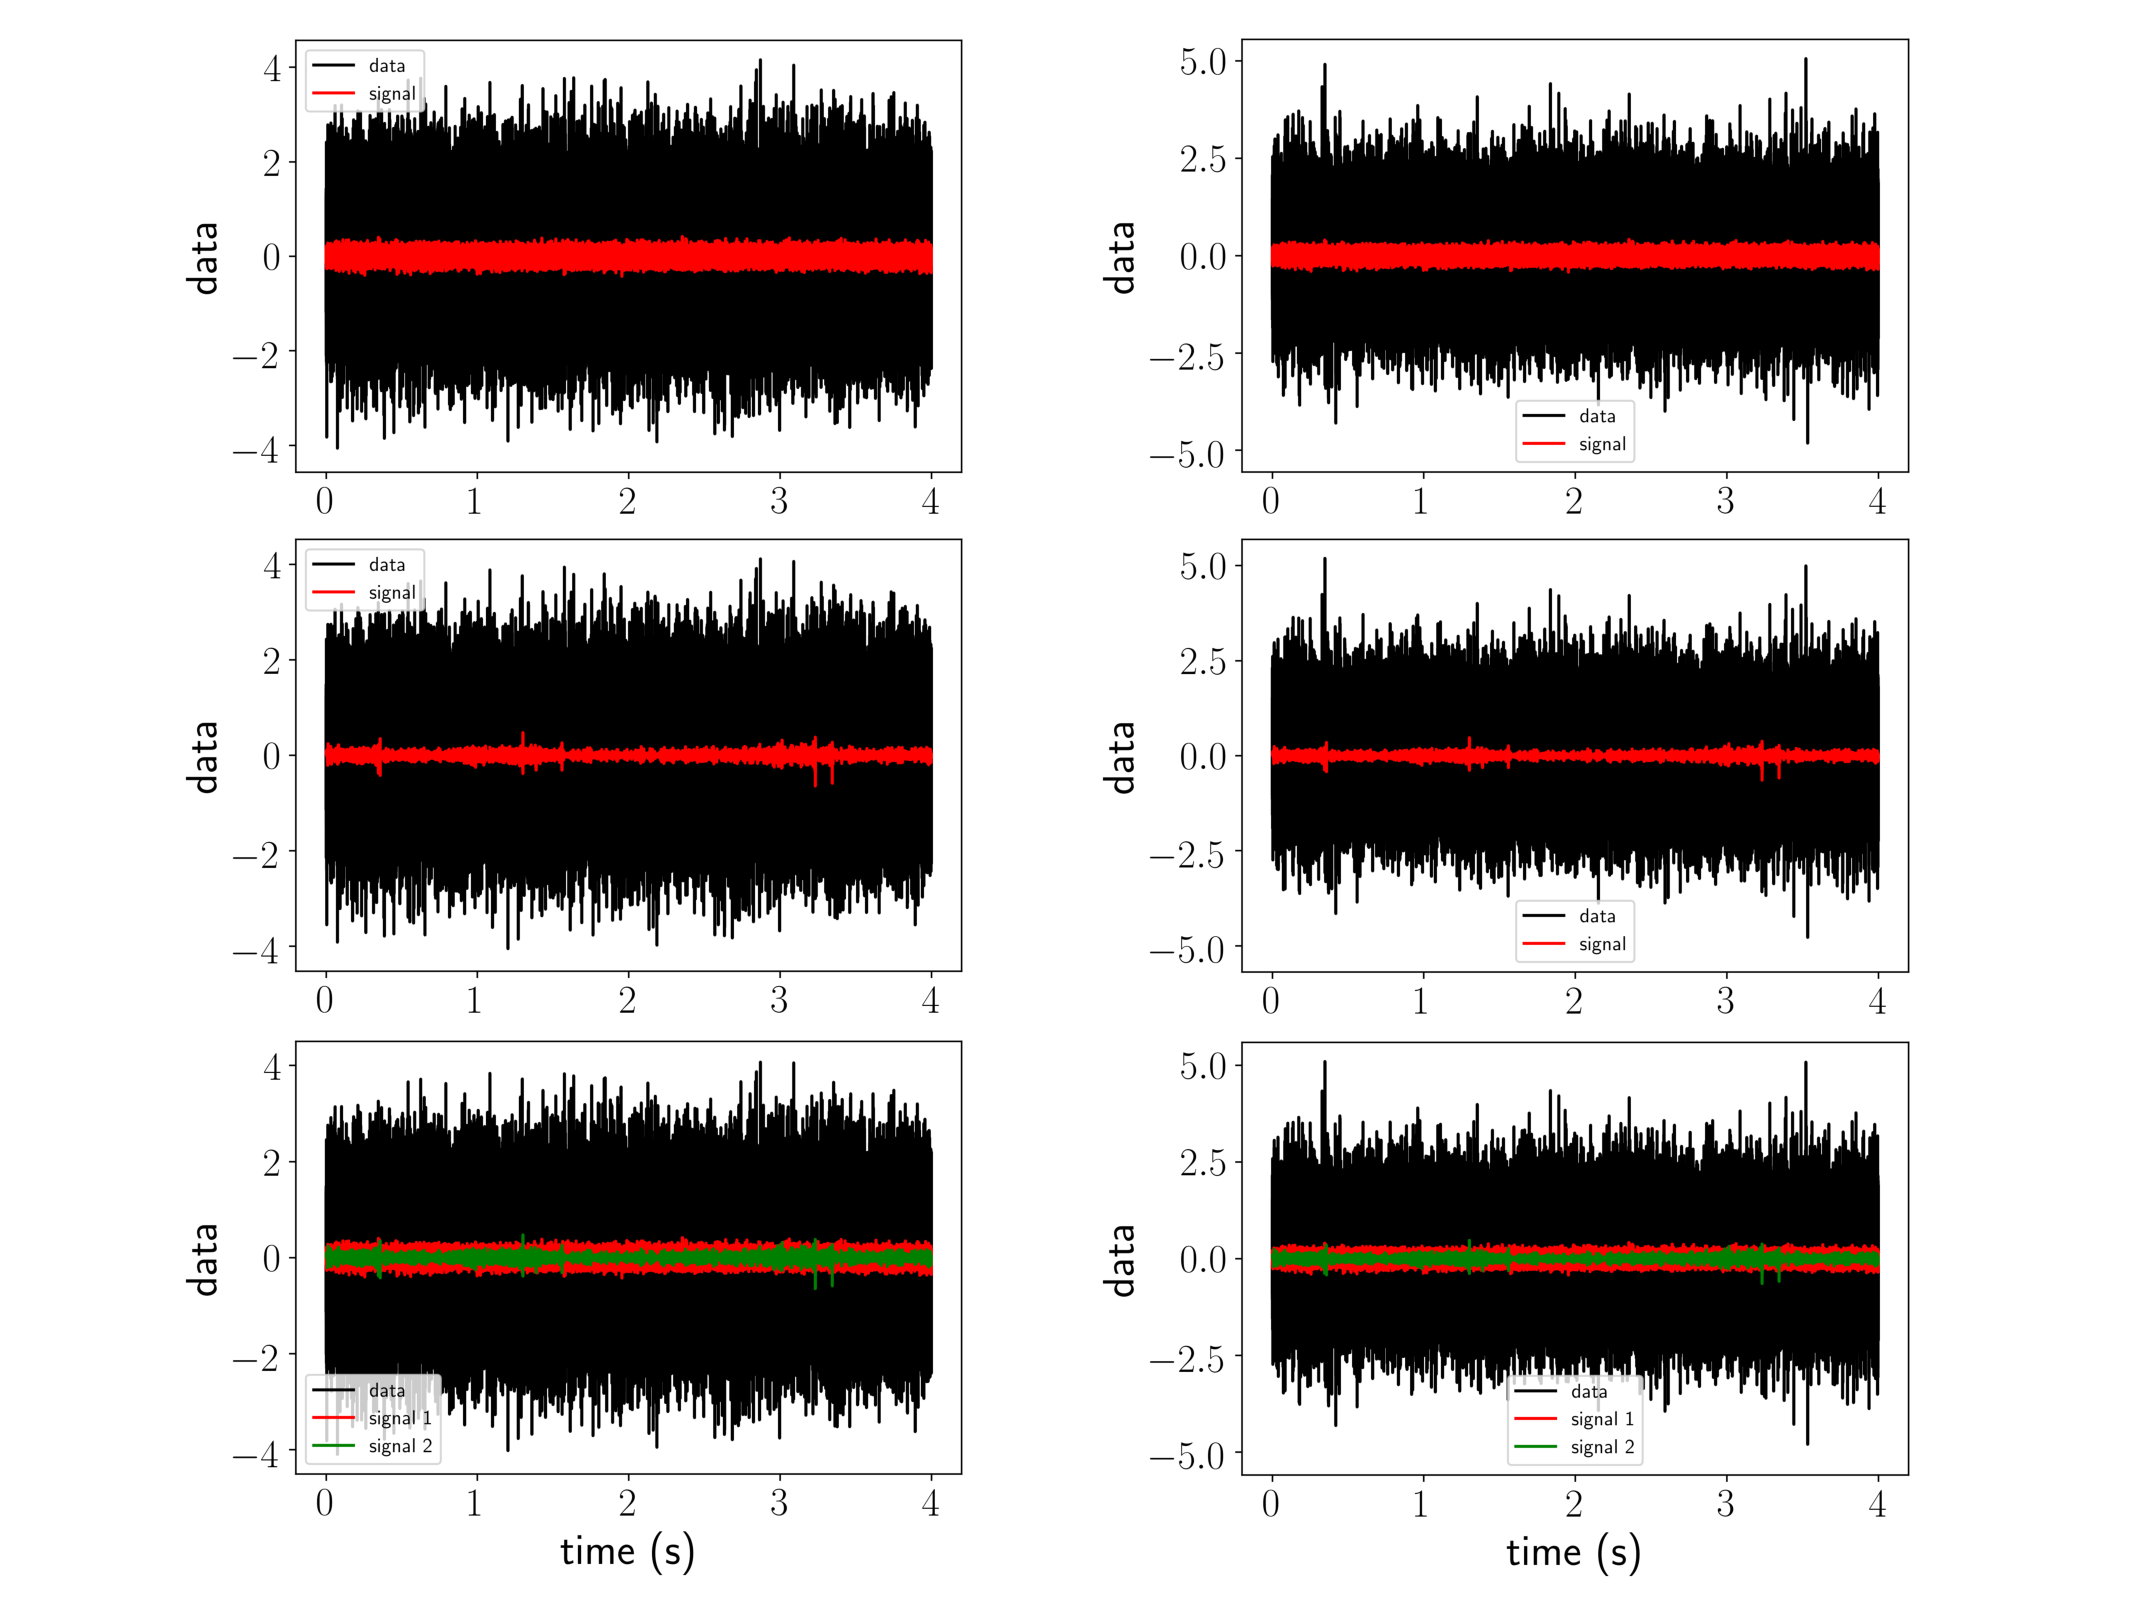
\includegraphics[width=\textwidth]{Figures/simple_examples}
\caption{Simulated time-domain data for the three different
cases discussed in the main text:
(top row) a white GWB in uncorrelated, white detector noise,
(middle row) a confusion-limited BNS background in uncorrelated, 
white detector noise,
(bottom row) a two-component background formed from the superposition 
of the GWBs from the top two rows in uncorrelated, white 
detector noise.
The two columns correspond to data in the two coincident
and coaligned detectors.
By eye one can see that signal components in the two detectors 
are identical, but the noise (and hence the data) in the two 
detectors are different.}
\label{f:simple_examples}
\end{center}
\end{figure}
%
Recall that a white GWB has a flat spectrum $H(f)=1$, 
while a confusion-limited background produced by BNS 
inspirals and mergers has spectral shape $H(f)=(f/f_{\rm ref})^{-7/3}$ 
(see Figure~\ref{f:different_power_spectra}).

\subsection{Single-component analyses}

We start by applying the single-component optimal-filter
analysis of the previous section.
For example (i), we find that the measured and injected
values of the amplitude of the GWB agree to 3.5\%, 
which is within 1-$\sigma$.
The corresponding optimally-filtered signal-to-noise
ratio is $\rho=2.9$.
For example (ii), the measured and injected values of
the amplitude of the GWB agree to 2.7\%, which again 
is within 1-$\sigma$.
The corresponding optimally-filtered signal-to-noise
ratio for this case is $\rho=12$.
Note that even though the overall amplitude of the
background is noticeably smaller for the confusion-limited
BNS background, the signal-to-noise ratio is considerably
larger (12 versus 2.9).
This is because the spectrum of the GW signal differs 
in this case from that of the detector noise,
which helps in distinguishing the signal and noise components.

Finally for example (iii), if we filter the data for 
the two components separately, 
we overestimate the amplitude of the white GWB component 
by 48\%, which is greater than 1-$\sigma$, and overestimate
the amplitude of the BNS background by 6.9\%, which is within 1-$\sigma$.
Basically, filtering the data for each GWB component 
separately typically leads to {\em overestimates}
of the amplitudes of the individual components, 
but {\em underestimates} of the error bars.
The overestimates arise since the other GWB component is
also contributing to the correlated signal.

\subsection{Multi-component analysis}

To better extract the amplitudes of the individual
components for example (iii), we need to go beyond 
single-component optimal-filtering, and consider 
a signal model that allows for a superpostion 
of multiple GWB components~\cite{Parida:2016}.
So instead of taking the cross-correlation to be a 
{\em single number}, $\hat C_{12}$, which is obtained 
by integrating the contributions from all 
frequencies, we will keep the frequency-dependence
explicit, defining
%
\be
\hat C_{12}(f)\equiv\frac{2}{T} \tilde d_1(f)\tilde d^*_2(f)
\,,
\ee
%
where $\tilde d_1(f)$, $\tilde d_2(f)$ are the Fourier
transforms of the time-domain data $d_1(t)$, $d_2(t)$ 
from the two detectors.
We will treat the values of $\hat C_{12}(f)$ 
for different frequencies $f$
as the `data points' from which to construct a 
{\em likelihood function}, which is the probability 
of the data given the parameters defining the signal
and noise models.%
\footnote{See John Veitch's lectures in this Volume
for more details regarding likelihood functions and
Bayesian inference.}
For this case, the signal model is given by the expected 
value of the correlated data:
%
\be
\langle\hat C_{12}(f)\rangle
=\sum_\alpha \Gamma_{12}(f)A_\alpha H_\alpha(f)
\equiv \sum_\alpha M_\alpha(f) A_\alpha\,,
\ee
%
where $H_\alpha(f)$ are the different spectral
shapes having amplitudes $A_\alpha$.
(Abstractly, we can think of $M_\alpha(f) \equiv
\Gamma_{12}(f) H_\alpha(f)$ as a matrix with indices
$f$ and $\alpha$, where $f$ runs over different 
frequency bins and $\alpha$ runs over different 
spectral components.)
The noise model enters via the covariance matrix 
of the data:
%
\be
N_{12}(f,f') 
\equiv \langle \hat C_{12}(f)\hat C_{12}^*(f')\rangle -
\langle \hat C_{12}(f)\rangle \langle \hat C_{12}^*(f')\rangle
\simeq \delta_{ff'}\,P_1(f) P_2(f)\,,
\ee
%
which is the product of the noise power spectra
in the two detectors in the weak-signal approximation.
The likelihood function is then%
\footnote{We are using here an {\em index-free} matrix notation, 
dropping the $\alpha$, $\beta$, $f$, and $f'$ indices, 
as well as the sums and integrals 
over $\alpha$ and $f$.
If we explicitly insert all of the indices, 
sums, etc., the argument of the exponential becomes
$$
-\frac{1}{2}\int_{-\infty}^\infty \D f
\frac{|\hat C_{12}(f)-\sum_\alpha M_\alpha(f)A_\alpha|^2}
{P_1(f)P_2(f)}\,.
$$}
%
\be
p(\hat C|A,N)\propto\exp\left[-\frac{1}{2}
(\hat C-MA)^\dagger N^{-1}(\hat C-MA)\right]\,,
\ee
%
which is the probability of the cross-correlated data
$\hat C_{12}(f)$ 
given the amplitudes $A_\alpha$ of the GWB 
spectral components 
and the noise in the two detectors $N_{12}(f,f')$.

We can now obtain estimators of the amplitudes of the 
GWB components, by maximizing the likelihood function 
with respect to the $A_\alpha$.
The final result (which you are asked to show in 
Exercise~\ref{exer:5}) is: 
%
\be
\hat A = F^{-1} X\,,
\ee
%
where
%
\be
F\equiv M^\dagger N^{-1} M\,,
\qquad 
X\equiv M^\dagger N^{-1} \hat C\,.
\ee
%
The quantity $F$ is called the 
{\em Fisher information matrix}.
In terms of its components,
%
\be
F_{\alpha\beta} = \int_{-\infty}^\infty \D f\> \frac{H_\alpha(f)\Gamma_{12}^2(f)H_\beta(f)}
{P_1(f)P_2(f)}\,.
\ee
%
Thus, we see that the Fisher matrix is a noise-weighted 
inner product 
of the spectral shapes $H_\alpha(f)$, $H_\beta(f)$ with one 
another.
Provided the spectral shapes are not degenerate (i.e., not 
propoportional to one another), then the Fisher matrix $F$
can be inverted and $\hat A$ calculated.
Otherwise, some form of regularization is needed to 
perform the matrix inversion.
The inverse of the Fisher matrix, $F^{-1}$, turns out to
equal the covariance matrix of the estimators $\hat A$.  

Using the above multi-component formalism, we are now able 
to extract the ampltitude of the white GWB component to 7.3\%, 
corresponding to a signal-to-noise ratio of 1.4, 
and to extract
the amplitude of the BNS background component to 3.8\%,
corresponding to a signal-to-noise ratio of 6.0.
In essence, the {\em joint} multi-component analysis 
properly takes into account the {\em covariance}
between the spectral shapes of the two components, 
allowing for unbiased, minimal variance estimates of 
the amplitudes $A_\alpha$.

